\documentclass[twoside,openright,a4paper,papersize,uplatex,dvipdfmx]{jsbook}
% uplatex オプションを指定し、ユニコード対応に。ただだし、uplatex でコンパイルすること。

% 修論本体と表紙で共通で必要となる設定
% jsbookで余白が広すぎるのを直す
% 参照 https://oku.edu.mie-u.ac.jp/~okumura/jsclasses/
\setlength{\textwidth}{\fullwidth}
\setlength{\evensidemargin}{\oddsidemargin}
\addtolength{\textwidth}{-5truemm}
\addtolength{\oddsidemargin}{5truemm}

% 同梱の ISEE 用の表紙テンプレ
\usepackage{thesis_cover}

% OTF フォントを使えるようにし、複数のウェイトも使用可能にする。
% これがないと、Mac のヒラギノ環境で使われる角ゴが太すぎてみっともない。
\usepackage[deluxe]{otf}
% OT1→T1に変更し、ウムラウトなどを PDF 出力で合成文字ではなくす
\usepackage[T1]{fontenc}
% uplatex の場合に必要な処理 
\usepackage[utf8]{inputenc} % エンコーディングが UTF8 であることを明示する。
\usepackage[prefernoncjk]{pxcjkcat} % アクセントつきラテン文字を欧文扱いにする
% Helvetica と Times を sf と rm のそれぞれで使う。
% default だとバランスが悪いので、日本語に合わせて文字の大きさを調整する。
\usepackage[scaled=1.05,helvratio=0.95]{newtxtext}
% 色
\usepackage[dvipdfmx]{color}
% 行番号を表示する。
\usepackage{lineno}

% latexdiff
% 実際の修論には入れる必要なし
%DIF PREAMBLE EXTENSION ADDED BY LATEXDIFF
%DIF UNDERLINE PREAMBLE %DIF PREAMBLE
\RequirePackage[normalem]{ulem} %DIF PREAMBLE
\RequirePackage{color}\definecolor{RED}{rgb}{1,0,0}\definecolor{BLUE}{rgb}{0,0,1} %DIF PREAMBLE
\providecommand{\DIFadd}[1]{{\protect\color{blue}\uwave{#1}}} %DIF PREAMBLE
\providecommand{\DIFdel}[1]{{\protect\color{red}\sout{#1}}}                      %DIF PREAMBLE
%DIF SAFE PREAMBLE %DIF PREAMBLE
\providecommand{\DIFaddbegin}{} %DIF PREAMBLE
\providecommand{\DIFaddend}{} %DIF PREAMBLE
\providecommand{\DIFdelbegin}{} %DIF PREAMBLE
\providecommand{\DIFdelend}{} %DIF PREAMBLE
%DIF FLOATSAFE PREAMBLE %DIF PREAMBLE
\providecommand{\DIFaddFL}[1]{\DIFadd{#1}} %DIF PREAMBLE
\providecommand{\DIFdelFL}[1]{\DIFdel{#1}} %DIF PREAMBLE
\providecommand{\DIFaddbeginFL}{} %DIF PREAMBLE
\providecommand{\DIFaddendFL}{} %DIF PREAMBLE
\providecommand{\DIFdelbeginFL}{} %DIF PREAMBLE
\providecommand{\DIFdelendFL}{} %DIF PREAMBLE
%DIF END PREAMBLE EXTENSION ADDED BY LATEXDIFF


%% 以下追加したpackage
% 画像の取り扱いに必要
\usepackage{graphicx}
% 数式の機能を拡張
\usepackage{amsmath}
\usepackage{bm}
\usepackage{upgreek}
\usepackage{newtxmath,newtxtext}
% コードを表示
\usepackage{listings}
\lstset{
    %プログラム言語(複数の言語に対応,C,C++も可)
    language = Python,
    %背景色と透過度
    backgroundcolor={\color[gray]{.98}},
    %枠外に行った時の自動改行
    breaklines = true,
    %自動改行後のインデント量(デフォルトでは20[pt])	
    breakindent = 10pt,
    %標準の書体
    basicstyle = \ttfamily\scriptsize,
    %コメントの書体
    commentstyle = {\itshape \color[cmyk]{1,0.4,1,0}},
    %関数名等の色の設定
    classoffset = 0,
    %キーワード(int, ifなど)の書体
    keywordstyle = {\bfseries \color[cmyk]{0,1,0,0}},
    %表示する文字の書体
    stringstyle = {\ttfamily \color[rgb]{0,0,1}},
    %枠 "t"は上に線を記載, "T"は上に二重線を記載
    %他オプション:leftline,topline,bottomline,lines,single,shadowbox
    frame = tbrl,
    %frameまでの間隔(行番号とプログラムの間)
    framesep = 5pt,
    %行番号の位置
    numbers = left,
    %行番号の間隔
    stepnumber = 1,
    %行番号の書体
    numberstyle = \tiny,
    %タブの大きさ
    tabsize = 4,
    %キャプションの場所("tb"ならば上下両方に記載)
    captionpos = t
}
% 複数引用
\usepackage{cite}
%\usepackage{natbib}
% 複数図を並べる時のcaption
\usepackage{subcaption}
\usepackage{here}
% 表関連
\usepackage{booktabs}
% 表でセルを複数列で結合する
\usepackage{multicol}
\usepackage{multirow}
% PDF 内で外部リンクや文書内リンクを生成したい場合に使う(好みによる)
\usepackage[dvipdfmx, hidelinks]{hyperref}
\usepackage{url}
% 複数行コメント
\usepackage{comment}
% 番号付き箇条書きのオプション利用
\usepackage{enumerate}
% renewcommandなどはここに
\usepackage{mymacros}
% 目次でsubsectionまで表示
\setcounter{tocdepth}{2}



% 画像の取り扱いに必要
\usepackage{graphicx}


% 数式の機能を拡張
\usepackage{amsmath}
\usepackage{bm}
\usepackage{upgreek}

% 複数引用
\usepackage{cite}


% 複数図を並べる時のcaption
\usepackage{subcaption}
\usepackage{here}

% 表関連
\usepackage{booktabs}
% 表でセルを複数列で結合する
\usepackage{multicol}
\usepackage{multirow}
% 行番号を表示する。添削時のみに使い、事務提出版ではコメントアウトする
%\usepackage{lineno}
%\linenumbers

% PDF 内で外部リンクや文書内リンクを生成したい場合に使う(好みによる)
\usepackage[dvipdfmx, hidelinks]{hyperref}



% renewcommandなどはここに
\usepackage{mymacro}
% 目次でsubsectionまで表示
\setcounter{tocdepth}{2}
% 複数行コメント
\usepackage{comment}


% 氏名などの情報が入っているファイル。各自で編集。
\title{深層学習による消化管腫瘍検出 \\ 〜3次元病理画像解析〜} % 論文題目
\date{2019年1月31日} % 日付(入れたくなければ空欄)
\heisei{31} % 年度
\StudentIdNumber{37-176484} % 学籍番号
\author{松崎  博貴} % 氏名
\seifuku{} % 正本か副本か(このファイルでは変更する必要なし)
% \labname{宇宙線物理学研究室} %
\supervisor{小野寺宏 特任教授} % 指導教員
\cosupervisor{染谷隆夫 教授} % 副指導教員


\begin{document}
% 式番号,図番号,表番号を章ごとの連番にする
\numberwithin{equation}{chapter}
\numberwithin{figure}{chapter}
\numberwithin{table}{chapter}


\frontmatter

\maketitle

% これを入れることでページ番号が表示されない。
\thispagestyle{empty}

% abstract 環境は jsbook では「概要」と表示してくれないため、手動で表示させる。
% 参照 http://oku.edu.mie-u.ac.jp/tex/mod/forum/discuss.php?d=2121
\begin{center}
  {\large \sf 概要}
\end{center}

近年になって医療データが蓄積されるシステムができてきいる。医療画像をコンピューター上に取り込むようになってから、自動で解析するシステムを構築してきた。今までは、専門医が診断を行う場合は、判断が主観的であること、ミスをする可能性があること、専門化同士でも意見が異なること、実際の臨床現場で医師はたくさんの画像を処理しなくてはいけないので、1枚にかけられる時間が限られていることから、機械による診断支援システムが必要とされている。既存の機械によるルールベースによるシステムでは解析ルール人にバイアスがかかっているということや、画像認識の著しい精度向上があるディープラーニングを利用した方法によって解析する方法に注目されている。またコンピュータの計算性能と、ビッグデータである医療画像を処理する能力が向上した背景と重なって、現在は機械学習による医療画像解析の研究が盛り上がりを見せている。

\tableofcontents
\listoffigures
\listoftables

\mainmatter

% include を使うことで、別ファイルに分割することができます。
%\chapter{序論}
\label{chap_intro}
\section{けんきゆうはいけい}
胃がんは、日本でもっとも罹患数が多いがんであり、年間13万人が罹患し5万人が亡くなっている.内視鏡の生検は食道,大腸,小腸,胃などを鉗子で2mm角の立方体程度の大きさで抜き出し,染色したものを2,3断面にカットしてから病理診断医が顕微鏡で観察,診断している.
断面のみの観察では内部に腫瘍がある場合に見落としてしまうリスクがあるため,本研究では組織透明化技術を用いて検体を丸ごと観察できるようにした。病理医が全てを診断するには負担が大きいことと病変の見落としリスクがあること,経験を詰んだ医師でも判断の難しい病変を見つけることが求められている。

内視鏡で見つけた病変が、腫瘍か非腫瘍かを判別したり、その悪性度を判定することは生検を観察する必要がある.内視鏡検査の専門医のマンパワーが不足している.現在の日本の病理の専門医は2259名で,その人数に対して標本 500万件を年間で処理している現状である.

また癌検診では担当医が判定して専門医がダブルチェックをしているが,AIがスクリーニングを行って専門医の確認が必要な症例を絞り込む.専門医の判定は主観的であることや,専門医ごとにも判断基準がことなることが課題になる.

\begin{figure}[H]
	\centering
	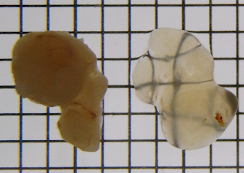
\includegraphics[width=0.7\linewidth]{fig/chapter1/lucid}
	\caption{transparent specimen}
	\label{fig:lucid}
\end{figure}

\begin{figure}[H]
	\centering
	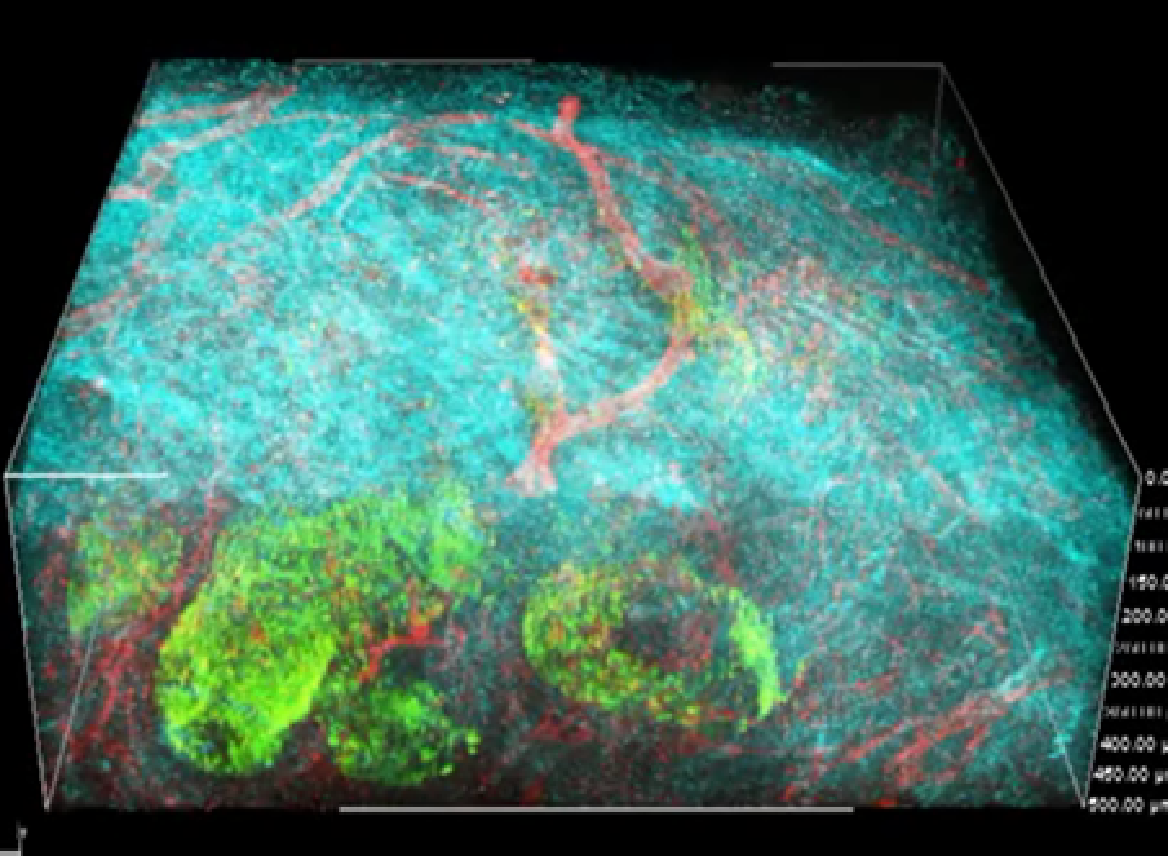
\includegraphics[width=0.7\linewidth]{fig/chapter1/microscope}
	\caption{microscope}
	\label{fig:microscope}
\end{figure}

\section{ほんけんきゆうのもくてき}
本研究の目的は内視鏡生検を透明にして深層学習を利用して癌を見落とさない診断方法を開発することである.組織透明化技術LUCIDを用いて検体を丸ごと透明化し,レーザー顕微鏡で観察することで,顕微鏡の解像度で検体の内部まで3次元情報として解析することができる.

\begin{figure}[H]
	\centering
	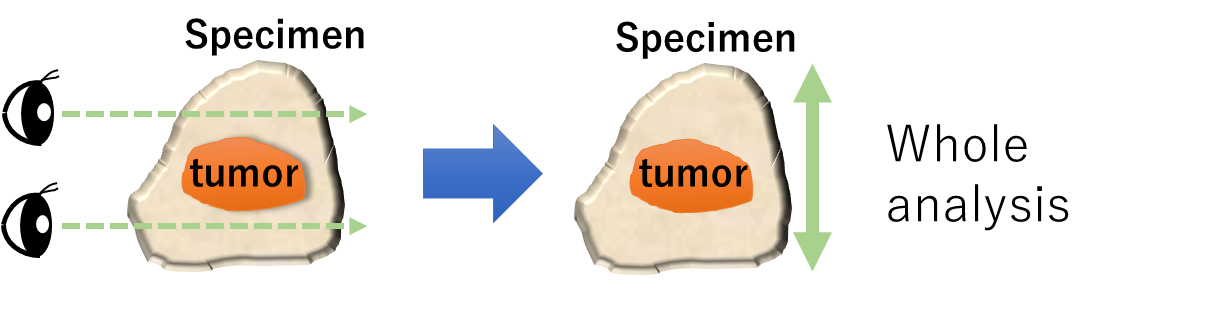
\includegraphics[width=0.7\linewidth]{fig/chapter1/whole_image_analysis}
	\caption{whole image analysis}
	\label{fig:wholeimageanalysis}
\end{figure}


透明化されたサンプルをレーザー顕微鏡で撮影すると,従来のカットする手法に換算して1000カットに相当するため,得られる顕微鏡撮影像が従来の2,3カットに対して数100倍となるので,専門医が診断をするには負担が大きくなってしまう.したがって,人工知能(Artificial Intelligence: AI)が3次元画像を解析して病変を検知し,専門医に提示することで病変の見落としリスクがゼロになる診断支援システムを開発することが本研究の目的である.

AIを用いた内視鏡の診断支援は生検ではなくて、内視鏡カメラの画像解析を行う事例がある。国立がん研究センターとNECが共同で開発したシステムがある。しかし、診断を確定するには生検が必須であり、生検の病理診断にマンパワーが必要になっている。生検のAIによる診断アルゴリズム開発の先行研究としては、胃がん、肺がんや乳がん、骨髄などの生検をディープラーニングで境界認識するものががあり、90\%程度の正解率を出して、専門医と同程度の精度がすでに達成されているものもあるがデータセットとして提供されているのは単純の形状のものが多い。本研究では生検の3次元画像を解析することで2次元画像では判断の難しいものを3次元特有の情報を用いることで判定精度を上げ、
機械学習を行うためには教師データを用意する必要があるが、医療データはアノテーションされていないことが多い。3次元画像を解析する先行研究としては、CTやMRI画像が上げられる。CTやMRIの場合は画像の分解能が顕微鏡像よりも低く、深さ方向にも30程度である。本研究は透明化処理した生検を蛍光顕微鏡で撮影するため分解能が高く、深さ方向にも400~700枚が撮影することができる。このためディープラーニングで解析するときに計算のメモリに乗らないという問題が生じるため解析手法を工夫して計算量がなるべく減るようにしなければいけない。今回は時系列処理で使われる手法と画像処理の手法を組み合わせて用いることで、大きな画像サイズでも解析することができるようにした。


深層学習で解析を行う場合はデータを大量に準備する必要がある.今回のように,新しい撮影手法であったり,希少な病気であったりすると医療データを数多く集められないことがある.さらに画像データだけでなく,その画像に教師ラベルを貼る(アノテーション)必要がある.画像と,その教師ラベルのセットを数万枚と集めることができたら高い精度が出るという報告が多くあるが,少ない教師データで識別精度を上げることは深層学習において困難とされている.教師データの作成が困難であるだけでなく,少量データである場合は,その教師データが医師によってばらつきがある場合は,教師データを作成した医師の判断が大きく反映されてしまい,必ずしも真であると断言することができなくなってしまう.これらの課題があるため医療画像における深層学習を用いた診断システムは,大量にデータを用意するまでの時間や人的コストを大きく払うことになっているのが現状である.

本研究でこの課題に取り組んだ.教師ラベルを必要とせず,画像の構造的な特徴のパターンを学ぶ,教師なし学習の手法と,これまでの教師ラベルを使った学習とを組み合わせた,半(弱)教師あり学習を行った.構造的なパターンは3次元画像であることを活用し,教師なし学習については,病理画像が正常から異常になる過程には連続的な性質があることを活用して正常と異常の分布が作れるようにした.


最後にこの深層学習による腫瘍の検出結果を医師が診断する際のサポートになるように可視化する.深層学習は,よく判断の理由が分からないためブラックボックスと呼ばれ,信頼性が求められる場面では利用に対して不安視されることがある.そのため腫瘍と正常の診断の判断の理由が可視化して,どの部分に注目しているかを医師に見せる.医師の負担を減らすためのスクリーニングとして利用するために,明らかに正常のものと,腫瘍かもしれない領域とを区別して,腫瘍かもしれない部分を医師に提示する.3次元画像であるから医師が診断するには,全ての断面を確認することは現実的に不可能である.腫瘍を見落とさないように,深層学習によって,腫瘍がある確率の高い断面を提示して診断支援を行う.
 % 背景
\chapter{深層学習による病理画像の診断支援}
\label{chap_review}

病理画像をデジタルで保存することが始まったのは数十年前になる.これによって遠隔地でも診断することができるようになったり,情報を共有することができるようになり,複数の医師で診断しミスを防止するセカンド・オピニオンが容易になった.計算機科学の分野の側面ではデータを収集することができるようになり,研究が盛んに行われることになった.その後は,様々な病理データでより改良されたアルゴリズムの提案が行われている.

細胞組織の形態を観察するための病理染色ではヘマトキシリン・エオジン染色(HE染色)が一般的に用いられる.細胞核を青紫色に染色し,細胞質をピンク色に染色する.正常から異常に変化していくと,細胞核が過度に増殖したり,細胞質の形が崩れたりすることで,その特徴を機械学習によって精度よく検出するための研究が行われている.

これまでは,核の形やテキスチャーからパターンマッチングなどの画像処理によって腫瘍を検出する研究されてきたが,近年になって画像処理に大きなブレークスルーが起きたことをきっかけに,新しい手法で解析するようになってきた.そのブレークスルーがディープラーニングである.

\section{ニューラルネットワーク}\label{sec:NeuralNetwork}
人間の脳にはニューロンと呼ばれる神経細胞が1000億個以上あり,それぞれが複数のニューロンが電気信号によって情報を伝達している.また脳にはシナプスという場所があり,ここで電気信号を細胞体へ受け渡す.細胞体はある閾値以上の電気信号がきた場合に他のニューロンへ電気信号を伝播させる(これを発火と呼ぶ).このようなニューロンとシナプスで行われる演算を模倣したアルゴリズムを作ることができれば,人間のような思考や認識をコンピュータを使って再現できると考えた.そのアルゴリズムがニューラルネットワーク(Neural Network: NN)である.

\subsection{多層パーセプトロン}
ニューラルネットワークは入力層,出力層,隠れ層から構成され,層と層の間にはニューロン同士のつながりの強さを示す重みがある.非線形問題を扱うために1986年Rumelhartによって考案されたのが,パーセプトロンを複数つなぎ合わせ入力と出力以外に隠れた層を持つ多層パーセプトロン(Multi-layer perceptron: MLP)である(\fig {mlp}).ニューラルネットワークで多層パーセプトロンの層を全結合(fully connected: FC)層とも呼ぶ.

\begin{figure}[H]
	\centering
	\begin{minipage}[b]{0.4\columnwidth}
		\centering
		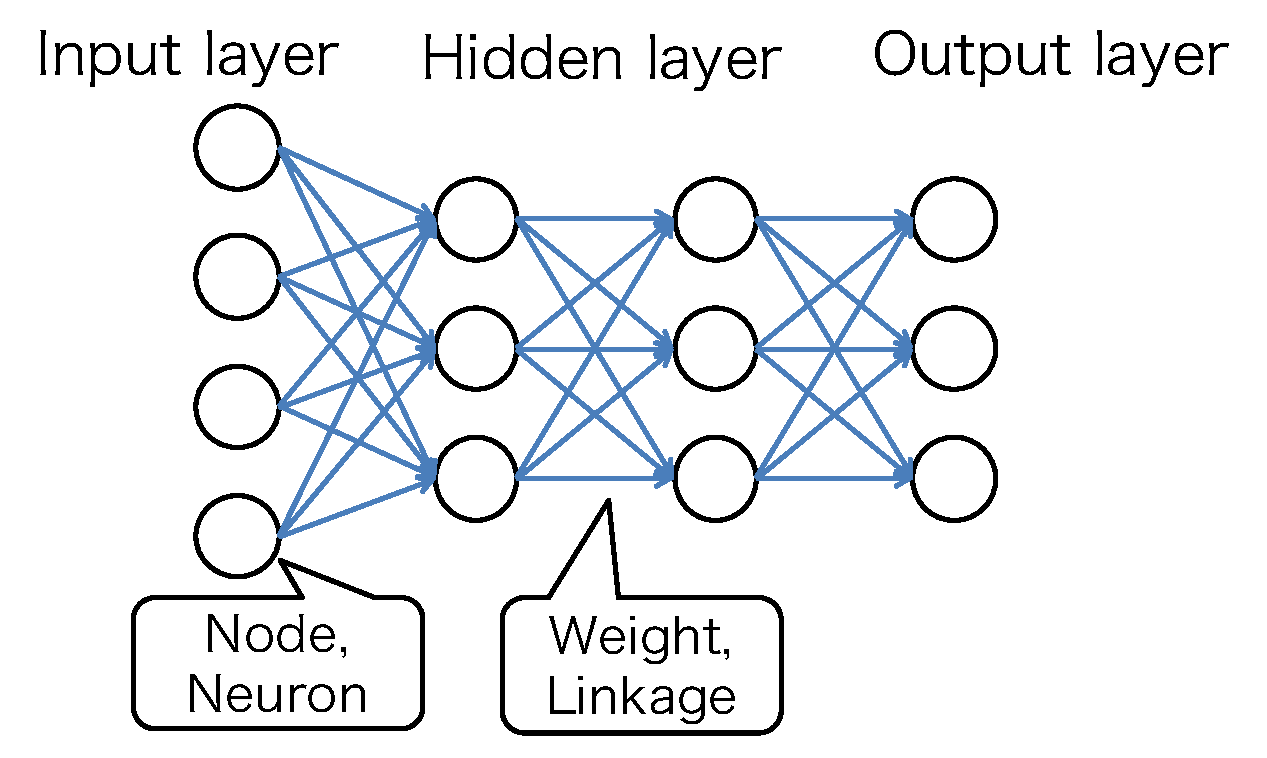
\includegraphics[width=1.2\linewidth]{fig/MLP}
		\subcaption{Muti-layer perceptron}
		\label{fig:mlp}
	\end{minipage}
	\begin{minipage}[b]{0.4\columnwidth}
		\centering
		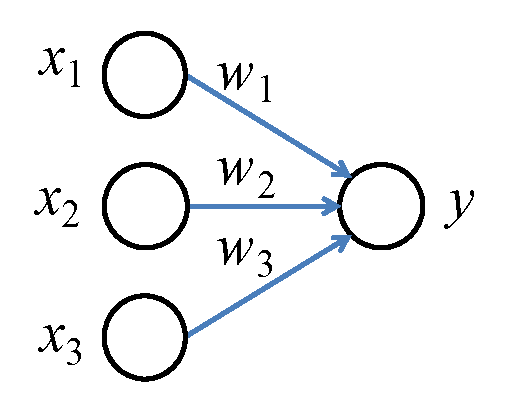
\includegraphics[width=0.7\linewidth]{fig/simple_perceptron}
		\subcaption{Simple perceptron}
		\label{fig:perceptron}
	\end{minipage}
	\caption{Architecture of Muti-layer perceptron}
\end{figure}

\fig {mlp}における丸や矢印はそれぞれノード(またはニューロン)と重み(または結合)と呼び,ともに数値である.例えば画像を分類しようと思えば,各ピクセルの画素数を各ノードに入力する.例えば$28 \times 28$pixelのグレースケール画像であれば,784個のノードが必要となる.入力データ$\bm {x}$が入力層に入ってくると,その値に重み$\bm {w}$をかけ,活性化関数$H$と呼ばれる関数に通し,結果$\bm{y}$を出力する.ここで,入力$\bm{x}$,重み$\bm{w}$,出力$\bm{y}$を太字で表したが,これらは全てテンソルであり,1つの層にあるノード$x_1, x_2, \cdots x_n$を一括して$\bm {x}$として表記している.

ここで,中間層の1つのノードについて考える.\fig {perceptron}にMLPを構成する1ユニットである単純パーセプトロンを示した.この模式図を数式で表すと次のようになる.
\begin{align}
	y & = H(\bm{w}\bm{x} + \bm{b}) \\
	& = H\left( \sum_{i=1}^3 w_i x_i + b_i \right) 
\end{align}
ここで$\bm{b}$はバイアスと呼ばれ,発火のしやすさを表している.中間層における活性化関数は,\eq {ReLU}に示す正規化線形関数(rectified linear unit: ReLU)と呼ばれる関数)がよく用いられる.
\begin{align}\label{eq:ReLU}
	H(x) = \max \left\lbrace 0, x \right\rbrace = \begin{cases}
	x & (x > 0) \\
	0 & (x \leq 0)
	\end{cases}
\end{align}
この演算を繰り返し出力層に書き出す.ここで,各層の重みの値によって出力結果は異なってくる.

出力層では,ノードの個数は区別したいクラス数分用意する.
各ノードの出力値が各クラスに属している確率を表すように,活性化関数にはソフトマックス関数を用いる(ただし二値分類の場合はシグモイド関数を用いる).ソフトマックス関数は\eq {softmax}で表される.
\begin{align}\label{eq:softmax}
	y_i = \dfrac{\exp(x_i)}{\displaystyle \sum_{k=1}^n \exp(x_k)}
\end{align}
ここで$y_i$は,出力層が全部で$n$個あるとして,$i$番目の出力であることを示す.\eq {softmax}からわかるように,入力の総和に対して1つのノードがどれくらいの値を持つかという割合で表されている.これにより各ノードの出力は確率として解釈できるため,値の一番大きいノードのインデックスを予測ラベルとして見ることができる.


\subsection{畳み込みニューラルネットワーク}
従来の画像認識では,画像から特徴を抽出しそれを識別器にかける手法が主流であった.古典的手法では画像から特徴を抽出するいわゆる特徴量設計が必要で,ここをいかにうまく設計するかがポイントであった.特徴抽出の方法として,HOG\cite{HOG}やSIFT\cite{SIFT},SURF\cite{SURF}などがあり,これらによって抽出した特徴ベクトルをSupport Vector Machine(SVM)\cite{SVM}によって識別することが多かった.

しかし,1998年にLeNetと呼ばれる畳み込みニューラルネットワーク(Convolutional Neural Network: CNN)が提案された\cite{LeNet}.CNNは畳み込み層とプーリング層からなっている.この畳み込みとプーリングの演算を通して,特徴量設計から識別までをend-to-endで行うことができる.
\begin{figure}[H]
	\centering
	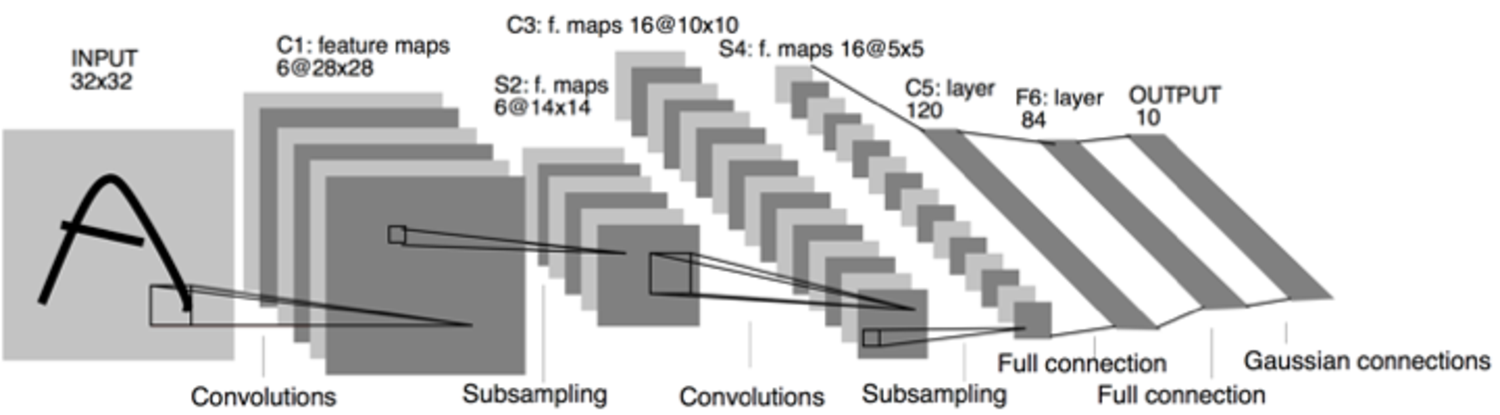
\includegraphics[width=0.7\linewidth]{fig/LeNet}
	\caption{Architecture of convolutional neural network\cite{LeNet}}
	\label{fig:LeNet}
\end{figure}


%人間が物体を認識することをコンピュータにも計算させるには,画像の特徴的な部分を切り分けて数値化させる必要がある.例えば,カラー画像の場合,RGBの3色(3チャンネル)を組み合わせた画像で認識をしている.このようなフィルターの畳み込み計算を行うと,フィルターごとに異なった画像の特徴を抽出して数値化する.これが畳み込み(convolution)である.その後,画像のサイズを小さくしてコンピュータが計算コストを減らし,微小な変化に対してロバストになる仕組みしてプーリングという方法を用いる.

畳み込み層では,入力に対してフィルター(カーネルとも呼ばれる)を用意し,\eq {conv}に示す計算を行う.
\begin{align}\label{eq:conv}
	y_{i,j} & = (\bm{K} * \bm{x})_{i,j}\\
	& = \sum_m\sum_n x_{i+m, j+n} K_{m,n}
\end{align}
ここで,$\bm{K}$はフィルター,$\bm{x}$は入力,$y$は出力である.CNNではこの演算の後に活性化関数に通す.これを図で表すと\fig {conv}のようになる.

\begin{figure}[H]
	\centering
	\begin{minipage}{0.45\columnwidth}
		\centering
		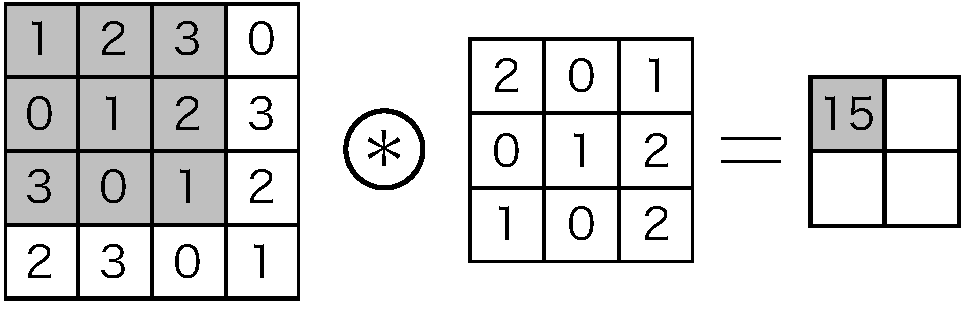
\includegraphics[width=\linewidth]{fig/conv_ex1}
		\subcaption{}
		\label{fig:conv_ex1}
	\end{minipage}
	\hspace{10truemm}
	\begin{minipage}{0.45\columnwidth}
		\centering
		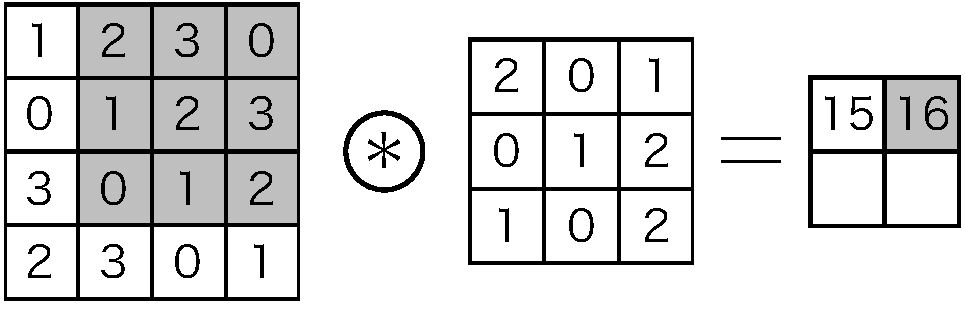
\includegraphics[width=\linewidth]{fig/conv_ex2}
		\subcaption{}
		\label{fig:conv_ex2}
	\end{minipage}
	\begin{minipage}{0.45\columnwidth}
		\centering
		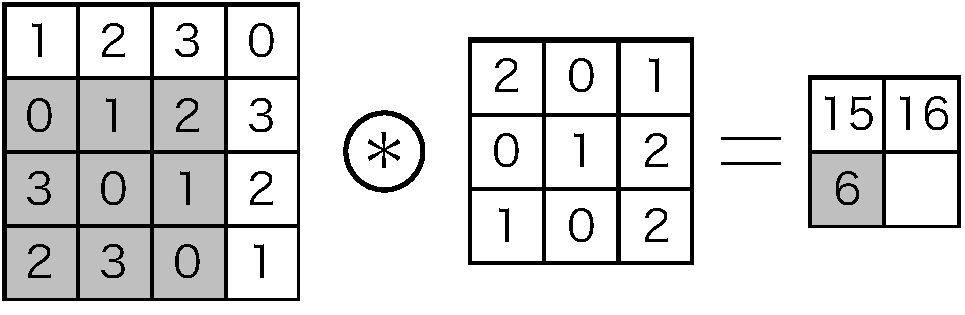
\includegraphics[width=\linewidth]{fig/conv_ex3}
		\subcaption{}
		\label{fig:conv_ex3}
	\end{minipage}
	\hspace{10truemm}
	\begin{minipage}{0.45\columnwidth}
		\centering
		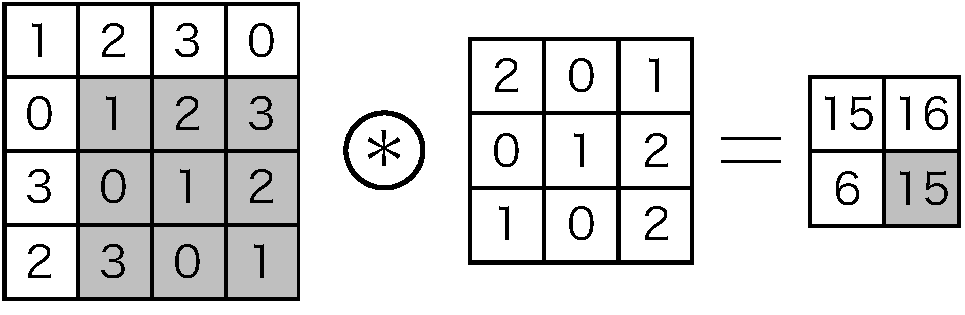
\includegraphics[width=\linewidth]{fig/conv_ex4}
		\subcaption{}
		\label{fig:conv_ex4}
	\end{minipage}
	\caption{Operation process of convolution}
	\label{fig:conv}
\end{figure}

\fig {conv}では,フィルターのサイズは$3\times 3$であるが,大きさは任意である($3\times 3$や$5\times 5$, $7\times 7$がよく用いられる).また,フィルターは1マスずつ横にずらして計算を行っている.ずらし方をストライドといい,今回はストライド1である.CNNでは多くの場合,ストライドは1である.
このようなフィルターの畳み込み計算を行うと,フィルターごとに異なった画像の特徴を抽出して数値化することができる.

次にプーリングを行う.ここでは,画像認識で多く用いられる最大値プーリングについて述べる.\fig {pooling}に示すように,$2\times 2$のプールサイズを用意した時,その範囲内にある最大値を取る演算である.ストライドはプールサイズと合わせ,プーリングを行った領域と被らないようにすることが一般的である.\fig {pooling}ではストライド2である.

\begin{figure}[H]
	\centering
	\begin{minipage}[b]{0.4\columnwidth}
		\centering
		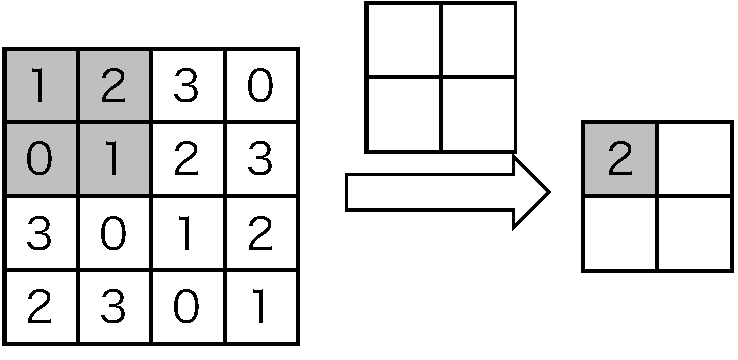
\includegraphics[width=\linewidth]{fig/pooling_ex1}
		\subcaption{}
		\label{fig:pooling_ex1}
	\end{minipage}
	\hspace{10truemm}
	\begin{minipage}[b]{0.4\columnwidth}
		\centering
		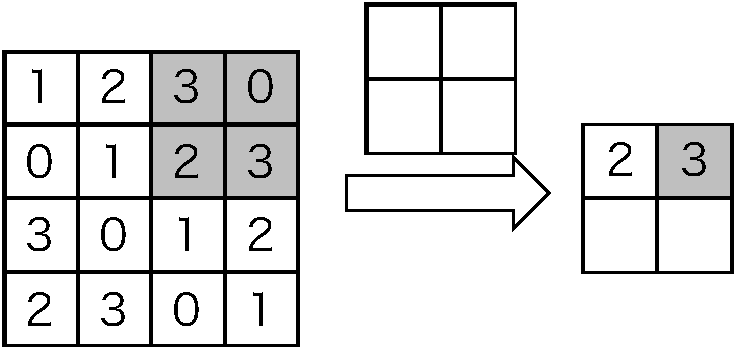
\includegraphics[width=\linewidth]{fig/pooling_ex2}
		\subcaption{}
		\label{fig:pooling_ex2}
	\end{minipage}
	\begin{minipage}[b]{0.4\columnwidth}
		\centering
		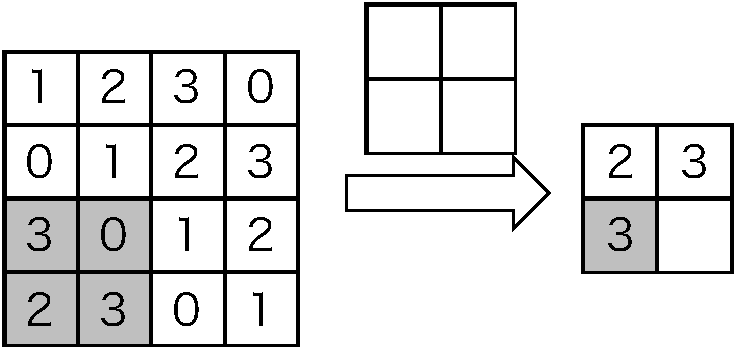
\includegraphics[width=\linewidth]{fig/pooling_ex3}
		\subcaption{}
		\label{fig:pooling_ex3}
	\end{minipage}
	\hspace{10truemm}
	\begin{minipage}[b]{0.4\columnwidth}
		\centering
		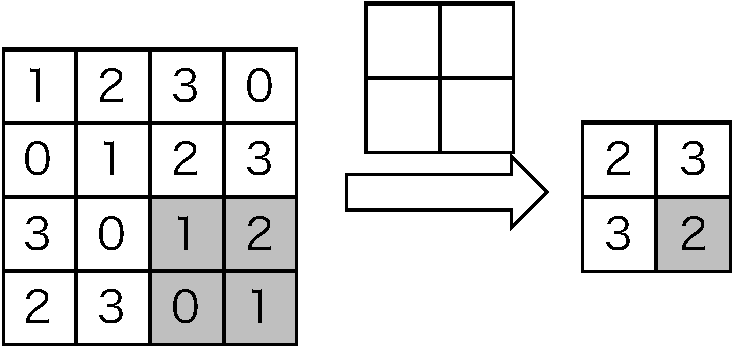
\includegraphics[width=\linewidth]{fig/pooling_ex4}
		\subcaption{}
		\label{fig:pooling_ex4}
	\end{minipage}
	\caption{Operation process of max pooling}
	\label{fig:maxpooling}
\end{figure}

プーリング層では画像のサイズを小さくして(コンピュータの)計算コストを減らし,微小な変化に対してロバストになる.

この畳み込みとプーリングを繰り返して,入力からフィルターの数だけ特徴を抽出し,この抽出した特徴マップをFC層へ繋げて識別を行う手法がCNNである.


\subsection{再帰的ニューラルネットワーク}
再帰的ニューラルネットワーク(Recurrent Neural Network: RNN)は時系列解析や自然言語処理に利用されるニューラルネットワークである.\fig {simpleRNN}に示すように,内部にループを持つことで過去の情報を保持しておくことができる.

\begin{figure}[H]
	\centering
	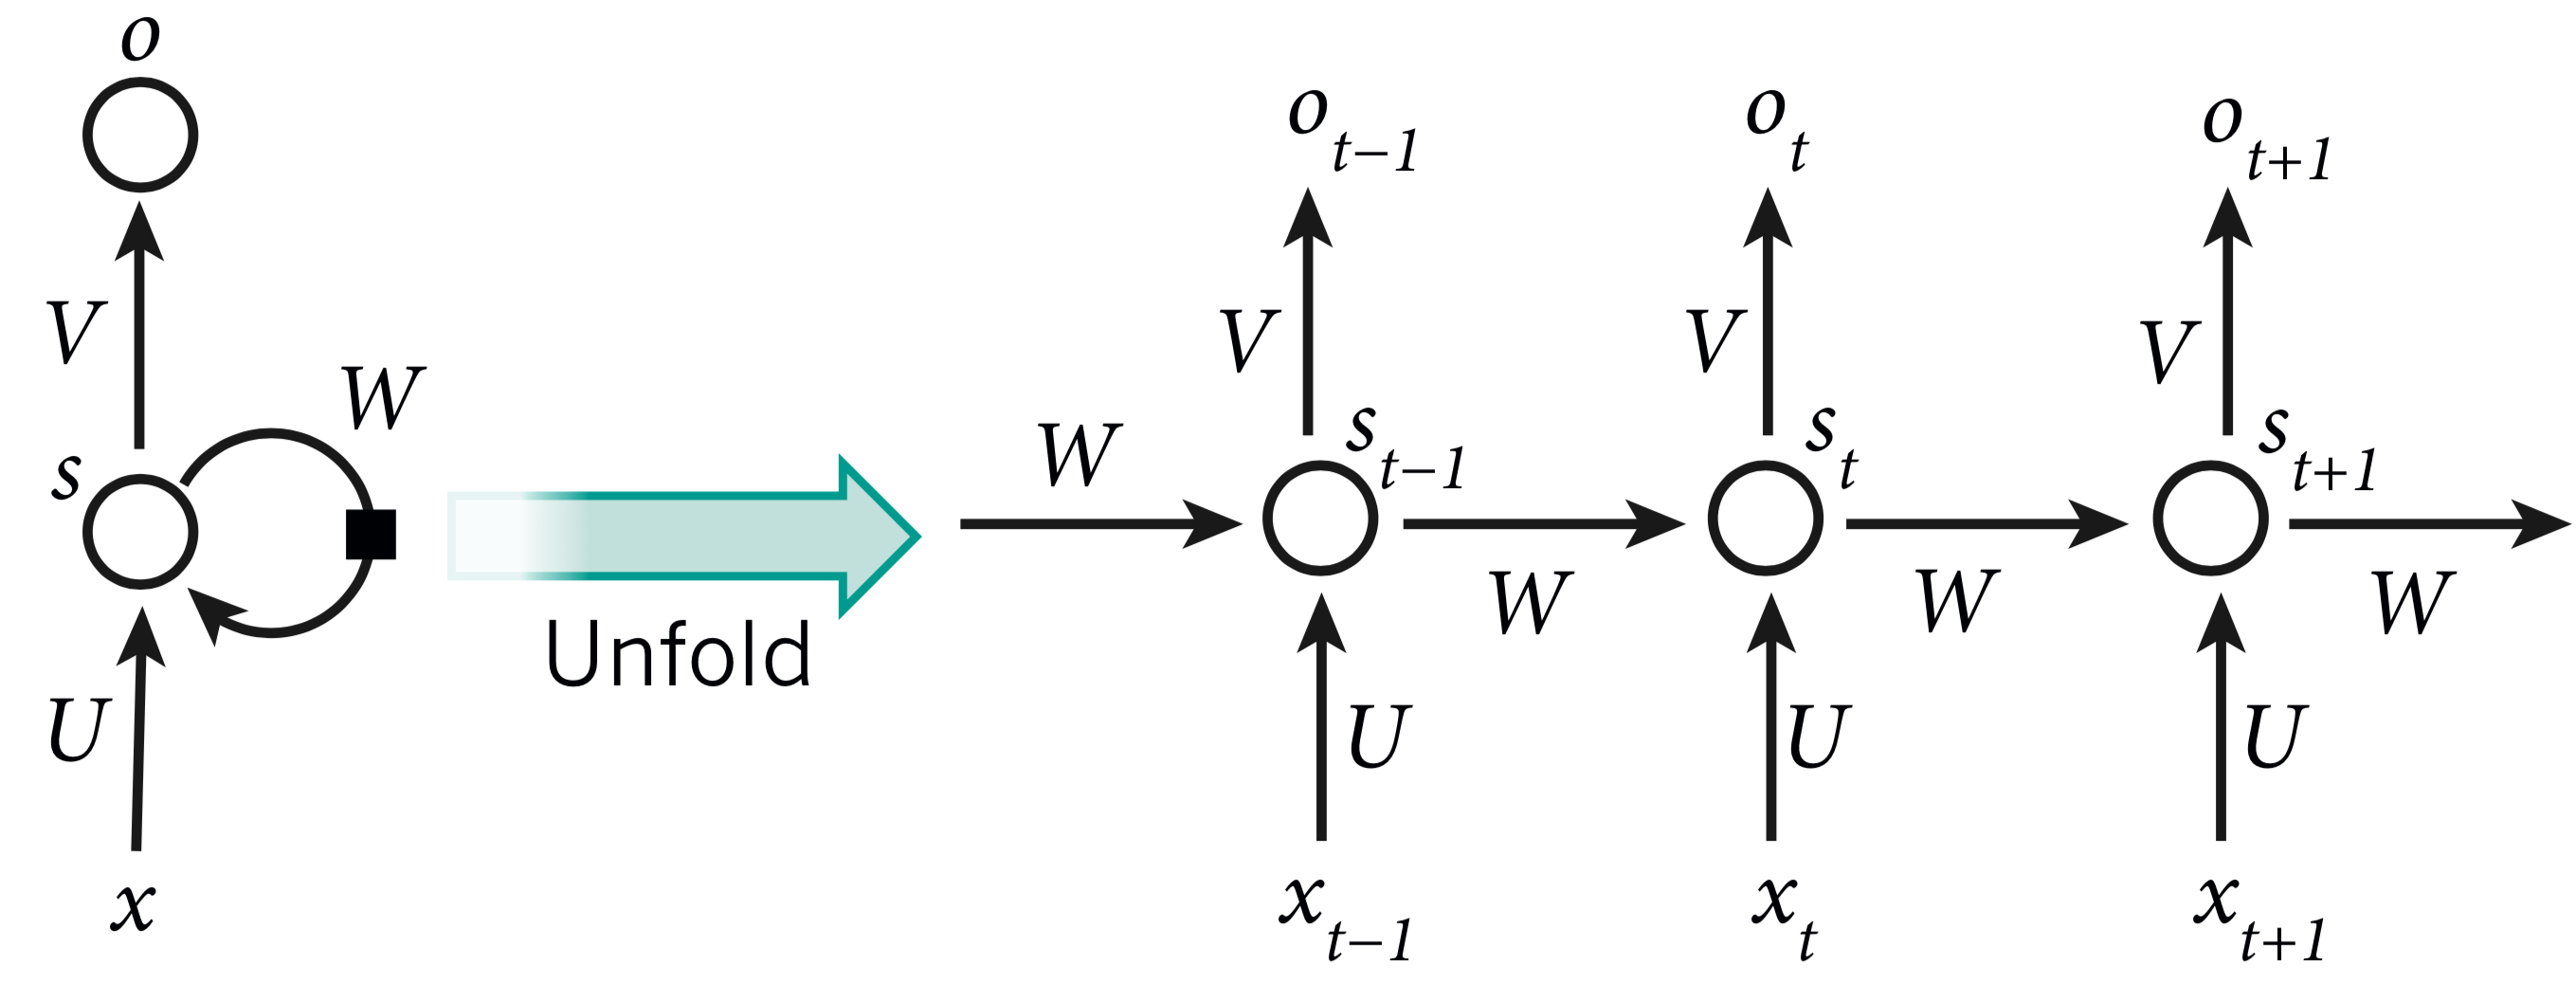
\includegraphics[width=0.7\linewidth]{fig/simpleRNN}
	\caption{Architecture of RNN\cite{simpleRNN}}
	\label{fig:simpleRNN}
\end{figure}


時系列の入力$\bm{x} = (x_1, \cdots , x_T)$があった時に,出力$\bm{y} = (y_1, \cdots , y_T)$と隠れ層のベクトル$\bm{h} = (h1, \cdots ,h_T)$をそれぞれ以下の式で計算する.

\begin{align}\label{eq:RNN}
	h_t & = H(W_{ih} x_t + W_{hh} h_{t-1} + b_h) \\ 
	y_t & = W_{ho} h_t + b_o
\end{align}

ここで,$\bm{W}$は重み行列($W_{ih}$は入力と隠れ層間の重み行列)であり,$\bm{b}$はバイアス項,$H$は活性化関数である.

\subsection*{LSTM}
RNNは,過去の情報をどこまで遡って関連性を見つけるか判断することができない.そのため,時系列データが長くなるほどその長期の依存性を学習するには人が慎重にパラメータを設計する必要があり,長期的なデータは学習が難しい問題があった.この問題を解決するためにLong-short term memory(LSTM)が提案された.\fig {LSTM}に示すように,LSTMもRNNの一種であるため繰り返し構造を持ち,3つのゲートを持つ層からなっている.

\begin{figure}[h]
	\centering
	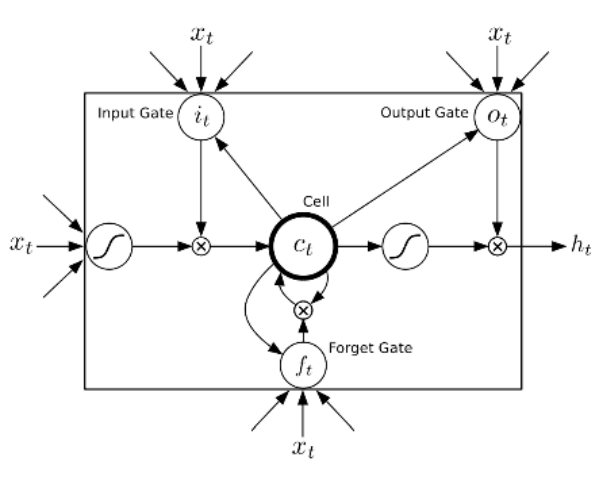
\includegraphics[width=0.7\linewidth]{fig/lstm.png}
	\caption{Architecture of LSTM}
	\label{fig:LSTM}
\end{figure}

\begin{align}\label{eq:LSTM}
	f_t & = \sigma(W_{xf} x_t + W_{hf} h_{t-1} + W_{cf} c_{t-1} + b_f ) \\
	i_t & = \sigma(W_{xi} x_t + W_{hi} h_{t-1} + W_{ci} c_{t-1} + b_i) \\
	c_t & = f_t c_{t-1} + i_t \tanh(W_{xc} x_t + W_{hc} h_{t-1} + b_c) \\
	o_t & = \sigma(W_{xo} x_t + W_{ho} h_{t-1} + W_{co} c_t + b_o) \\
	h_t & = o_t \tanh(c_t) 
\end{align}

ここで,活性化関数にはシグモイド関数および$\tanh$を用いる.シグモイド関数は次の式で定義される.
\begin{equation}\label{eq:sigmoid}
	\sigma (x) = \dfrac{1}{1 + e^{-x}}
\end{equation}

$f_t$で示される層は忘却ゲート層と呼ばれ,過去の情報で捨てるべき情報を判断する.これはシグモイド層によって行われ,0と1の間の値を出力し,0は完全に忘れる.1は完全に維持するという意味である.
$i_t$や$c_t$で示される層は,入力ゲート層と呼ばれ,$i_t$で新たに入力された情報から,どの情報を更新するかを判断し,$c_t$で古い情報を落とし新しい情報を加え値を更新する.
最後が$o_t$や$h_t$で示される層で,出力ゲート層と呼ばれる.まず何を出力するべきかを$o_t$のゲートで判断して,$c_t$に$\tanh$を適用して掛けることで出力が計算される.

\subsection*{GRU}


\section{推論と学習}
ニューラルネットワークでは推論フェーズと学習フェーズに分かれている.\ref{sec:NeuralNetwork}節は全て推論フェーズの話であり,順伝播ニューラルネットと呼ばれる.

学習フェーズでは,逆伝播ニューラルネットを用いる.逆伝播とは誤差逆伝播法(Backpropergation)\cite{Backprop}から由来している.真値からの誤差を表す損失関数(loss function)を用いて,パラメータの微分値を更新に用いる.損失関数はコスト関数,目的関数とも呼ばれる.この微分値を効率よく計算するアルゴリズムが誤差逆伝播法である.

損失関数は解く問題の目的に合わせて選ぶ必要がある.回帰問題では平均二乗和誤差(mean squared error: MSE)が用いられる.
\begin{align}\label{eq:mse}
	L_{\mathrm{MSE}} = \dfrac{1}{2} \sum_{k} (y_k - t_k)^2
\end{align}
また,クラス分け問題では交差エントロピー誤差(cross entropy error)が用いられる.
\begin{align}\label{eq:crossentropy}
	L_{\mathrm{cross}} = - \sum_k t_k \ln {y_k}
\end{align}
ここで,$y$は予測ラベルで,$t$は教師ラベルである.

\subsection{最適化手法}
損失関数を用いてパラメータを更新するが,更新手法にはいくつか方法があるため,ここでは本研究で使用した最適化手法について述べる.

\subsection*{SGD}
SGDは日本語で確率的勾配降下法(Stochastic gradient descent)と呼ばれる手法で,最も単純な最適化手法である.画像認識の分野では多く使われている.

SGDでは以下の式\eq {SGD}でパラメータを更新する.
\begin{align}\label{eq:SGD}
	\bm{W} \leftarrow \bm{W} - \eta \pdif{L}{\bm{W}} 
\end{align}
ここで,$\bm{W}$は更新する重みパラメータ,$\pdif{L}{\bm{W}}$は$\bm{W}$に関する損失関数の勾配である.また$\eta$は学習率と呼ばれ,実際には0.01や0.001といった値を前もって決めて使用する.SGDはパラメータの勾配を利用して,勾配方向にパラメータを更新するステップを繰り返して,徐々に最適なパラメータへと近づける手法である.

\subsection*{Adam}
Adam\cite{Adam}はadaptive moment estimationの略で,勾配の値の1乗和と2乗和の両方をパラメータ更新に用いる手法である.以下の式\eq{adam}でパラメータを更新する.

\begin{align}\label{eq:adam}
	\bm{m} & \leftarrow \beta_1 \bm{m} + (1 - \beta_1) \pdif{L}{\bm{W}} \\
	\bm{v} & \leftarrow \beta_2 \bm{v} + (1 - \beta_2) \left( \pdif{L}{\bm{W}} \right) ^2 \\
	\bm{W} & \leftarrow \bm{W} - \eta \dfrac{\hat{\bm{m}}}{\sqrt{\hat{\bm{v}}} + \epsilon} 
\end{align}

$m_t$と$v_t$はそれぞれ、勾配の一次モーメント(平均値)と二次モーメント(分散した平方偏差)の概算値である.$\eta$,$\beta_1$,$\beta_2$はそれぞれ学習パラメータである.
また,$\hat{m}_t$,$\hat{v}_t$はそれぞれ移動指数平均を用いた際に生じるバイアス(大きさを変えてしまっていることなど)を打ち消すために正則化しており,\eq {adamhat}で表される.

\begin{align}\label{eq:adamhat}
	\hat{\bm{m}} & = \dfrac{\bm{m}}{1 - \beta_1} \\
	\hat{\bm{v}} & = \dfrac{\bm{v}}{1 - \beta_2}
\end{align}

学習パラメータはそれぞれ$\eta = 0.001$,$\beta_1 = 0.9$,$\beta_2 = 0.999$,$\epsilon = 10^{-8}$が最適だと言われている\cite{Adam}.

\subsection{学習のテクニック}
ディープラーニングでは過学習(overfitting)と呼ばれる問題が多く起こる.過学習とは,訓練データに対してのみ適応し過ぎてしまい,訓練データに含まれないテストデータには精度が出ない状態を指す.過学習は,大量にパラメータを持つ表現力の高いモデルであることや,訓練データが少ないことなどが原因で起こる.ここでは過学習を抑制するテクニックを述べる.
\subsection*{Dropout}
Dropout\cite{Dropout}は,ネットワークのノードをランダムに消去しながら学習する手法である.訓練時に隠れ層のノードを毎回ランダムに選択し,そのノードの出力を0にする.そしてテスト時には全てのノードを活性化させ,信号を伝達させる.

Dropoutは,学習時にノードをランダムに消去することで,毎回異なるモデルを学習していると解釈でき,アンサンブル学習と同じ効果を擬似的に1つのネットワークで実現していると考えられる.アンサンブル学習とは,弱識別器を複数合わせて1つの強力な識別器とする手法で,現在でも有効な手法として用いられている.

\subsection*{Batch Normalization}
Batch Normalization\cite{BatchNorm}は,ネットワークにおける各層での活性化後の出力(アクティベーション)の分布を,適度な広がりを持つように調整する手法である.Batch Normalizationでは学習を行う際のミニバッチを単位として,ミニバッチごとに正規化を行う(\eq {BatchNorm}).
\begin{align}\label{eq:BatchNorm}
	\mu_B & = \dfrac{1}{m}\sum_{i=1}^m x_i \\
	\sigma_B^2 & = \dfrac{1}{m}\sum_{i=1}^m (x_i - \mu_B) \\
	\hat{x_i} & \leftarrow \dfrac{x_i - \mu_B}{\sqrt{\sigma_B^2 + \epsilon}}
\end{align}
ミニバッチとして$B = \{x_1, x_2, \cdots, x_m\}$という$m$個の入力データの集合に対して,平均$\mu_B$,分散$\sigma_B^2$を求め,入力データを平均0分散1となるように正規化を行う.$\epsilon$は0で除算されることを防ぐもので,極小の値を用いる.

Batch Normalizationを用いると,学習を速く進行させることができる,初期値にそれほど依存しない,過学習を抑制できるといった効果が期待できる.

\subsection*{Data Augumentation}
Data Augumentation(データ拡張)は,訓練データを人工的に水増しする手法である.例えば,入力画像に対して回転や縦横の移動,上下反転,鏡面反転などの操作をして訓練データを擬似的に増やす.これは,ニューラルネットは大きな位置ずれや対象物が回転した状態にあると別のものとして認識してしまうことを逆手にとった手法である.訓練データが少ないときに大きな効果を発揮する.


\section{画像認識におけるディープラーニング}
%教師あり学習であることもここで触れておきたい
Deep LearningとはDeep Neural Network(DNN)を指すことが多い.この"Deep"とは,ニューラルネットワークの層が深いことに由来している.

\fig {ImageNet}に画像認識タスクの精度の近年の推移を示す.これはImageNet Large Scale Visual Recognition Challenge (ILSVRC)と呼ばれる世界的な画像認識のコンペティションである(2010年から始まった).カテゴリ数は1000クラスで,画像枚数は120万枚の訓練データと15万枚のテストデータが用意されている.
\begin{figure}[H]
	\centering
	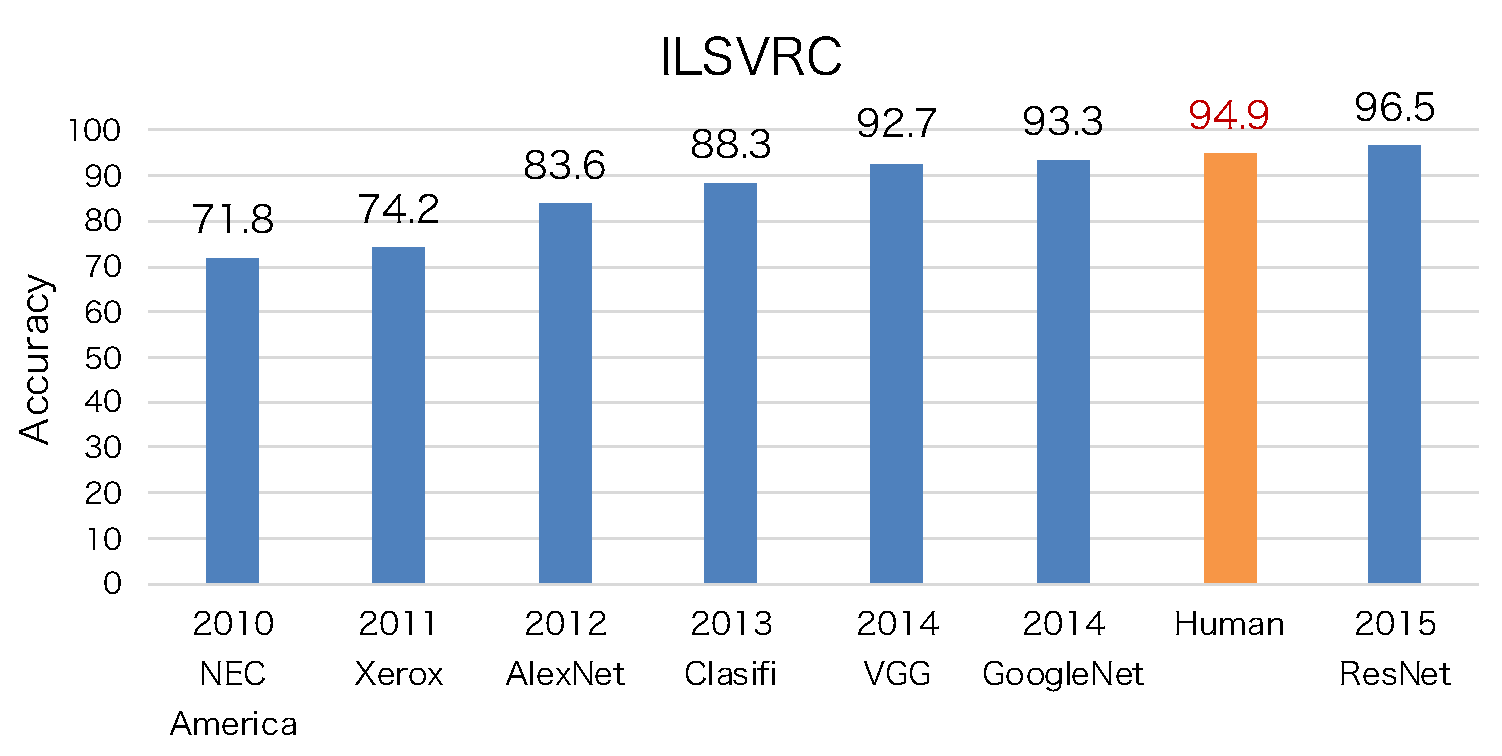
\includegraphics[width=0.7\linewidth]{fig/ILSVRC}
	\caption{Transition of accuracy of image recognition on ILSVRC}
	\label{fig:ImageNet}
\end{figure}
2011年と2012年は約10\%もの大差でAlexNet\cite{AlexNet}が優勝している.これがディープラーニングの始まりである.AlexNetは5つの畳み込み層と3つの全結合層を持っている.2014年にはVGGNet\cite{VGGNet}やGoogLeNet\cite{GoogLeNet}が9割の精度を超えた.VGGNetはAlexNet(8層)よりさらに深い構造(19層)であり,GoogLeNetは22層もある.そして2015年にはResNet\cite{ResNet}が人間の精度をも超える認識精度を達成した.ResNetはGoogLeNetよりもさらに深く152層もある.CNNを複数回かけて検出を行う場合,CNNの浅い側では空間分解能はあるが抽象的な情報が少ない.深い側では意味論的な情報は取得できる(ポーズ,変形など)が空間分解能が小さいため幾何学的な情報が失われる.

アーキテクチャの進化の方向は大きく3つある.1つ目は層を深くすることである.
2つ目はFC層の使用を避ける,またはInceptionモジュールの使用することである.これにより学習するパラメータ数を削減することができる.3つ目はResNetなどのショートカット接続の利用や,事前学習・転移学習を行うことである.これによって学習効率を向上させ,最終的にモデルの精度向上へと繋がる.ここで,事前学習のデータセットと適用データとの間には類似性があると良い.

画像処理におけるディープラーニングでは大きく3つのタスクがあり,それぞれ,クラス分類,物体検出,セグメンテーションである.以下に詳細を述べる.

\subsection*{クラス分類}
与えられた画像をカテゴリごとに分ける手法である.

\subsection*{物体検出}
物体検出とはBounding Boxで物体の位置とその物体の種類を特定する方法である.歴史的には幾何的情報,手動特徴量,そしてそのカスケードを利用していた.その後,HOGやSIFTなど局所特徴量を抽出する方法を設計するようになったが,これは深い専門知識を必要とした.また広い範囲でオブジェクトを正確に検出する方法は,メモリ容量と処理時間に課題がある.現在はDeep Neural Networkになりデータのみから抽象的な特徴量を複数得ることができる.\fig {YOLO}に物体検出で有名はアルゴリズムであるSSDとYOLOのアーキテクチャを示す.クラス分けの場合は数1000のカテゴリを学習してTop Error Rateが2\%以下と人間よりも認識精度が高いが,物体検出においては,現状ではカテゴリが数100程度くらいまででも認識精度が人間よりも低くなってしまう.また物体検出は精度を上げるために処理に時間がかかることが多いため,リアルタイムに物体検出を行う時は,速度と精度のトレードオフが生じてしまう.

\begin{figure}[H]
	\centering
	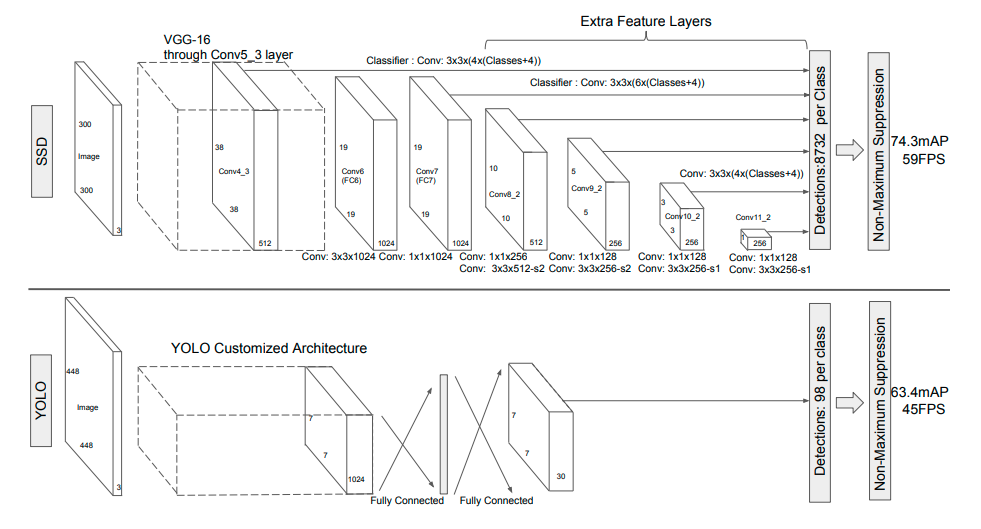
\includegraphics[width=0.7\linewidth]{fig/yolo_ssd.png}
	\caption{Network Architecture of SSD and YOLO}
	\label{fig:YOLO}
\end{figure}

\subsection*{セグメンテーション}
セマンティックセグメンテーションとは,画像を画素レベルで認識することである.画像内の各画素をオブジェクトクラスに割り当てる手法である.セマンティックセグメンテーションの手法についてディープラーニング以前では,Texton Forestsや,Random Forestsに基づいた分類を行っていたが,物体検出と同様にCNNが登場してからは,高精度なセグメンテーションが実現するようになった.CNNを使ったセグメンテーションの手法で一般的に使われるようになったものがUnetである(\fig {Unet}).このUnetは文字通りUの形をしたネットワークであることが特徴で,2つのアーキテクチャーからできている.1つ目がエンコーダーのアーキテクチャーでCNNとプーリングで特徴を抽出しながら次元を削減していき,2つ目のデコーダーのアーキテクチャーで画像をセグメンテーションの結果になるように復元する.ここで問題になることが,プーリングをすることで位置情報を消してしまっているので,この位置情報を利用して画像を復元するためには,エンコーダーとデコーダーで画像サイズが同じところ同士をショートカットで接続することがUnet構造の優れている点である.

\begin{figure}[H]
	\centering
	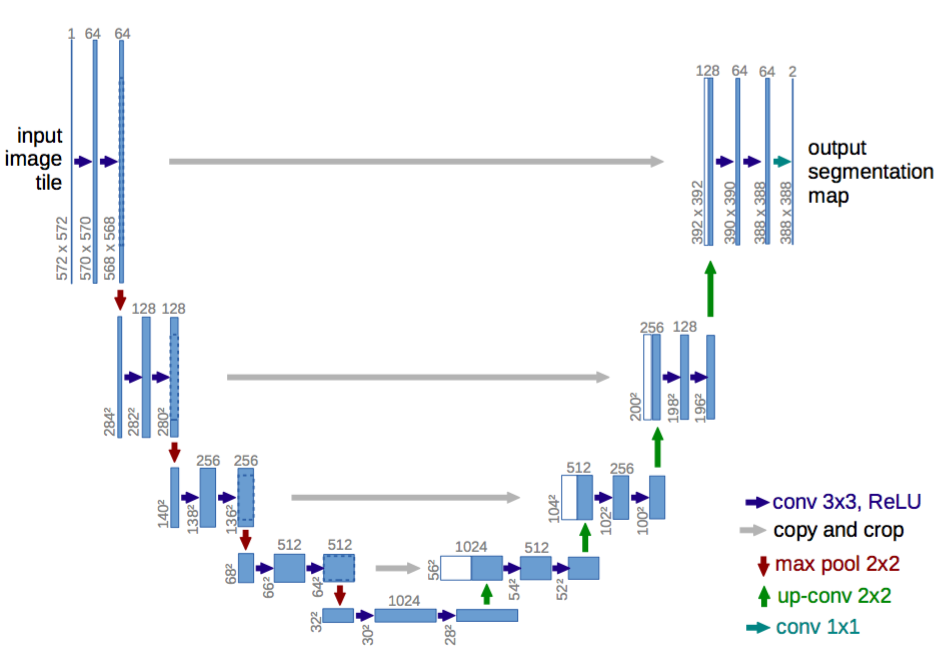
\includegraphics[width=0.7\linewidth]{fig/unet.png}
	\caption{Artchitecture of Unet}
	\label{fig:Unet}
\end{figure}

\section{深層学習による3次元画像解析}
ディープラーニングを医療画像に応用するコンペティションが世界で行われているが,その半数が3D医療画像の解析になっているほど需要が高まっている.その理由は,現在解決しなくてはならない課題があるからである.まずは2次元画像と違って,処理するべきデータが大きいということである.そのため学習するパラメータをなるべく少なくする工夫がされている.また3次元画像には,動画または,ボリューム画像があるが,2次元画像とその深さ方向(動画であれば,時間方向)には異方性があることから,機械学習の方法に工夫が必要になる.今まで考案されている手法として,2DCNNを拡張した3DCNN,またCNNと時系列解析でよく用いられるLSTMを組み合わせた手法と,LSTM内部にCNNを組み込んだ手法,それらをすべて組み合わせた手法が考案されいる.LSTMの研究も盛んに行われているため,その改良モデルが数多く存在する.特に,LSTMの学習効率を上げたGRU(Gated Linear Unit)や,順方向だけでなく逆方向の時系列も計算に入れるBiLSTMが時系列解析の精度向上になっている報告がある.


\subsection{3DCNNとStacked Convolution}
2次元画像が深さ方向に連続している3次元画像の特徴を抽出するために,2次元のCNNを拡張して,3次元のカーネルを使って畳み込みを行う,3DCNNを利用した手法がある.

\begin{figure}[H]
	\centering
	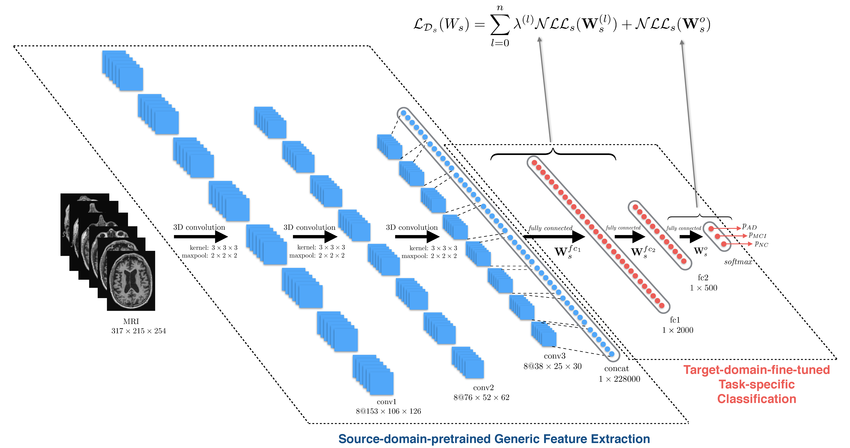
\includegraphics[width=0.7\linewidth]{fig/3d_cnn.png}
	\caption{Artchitecture of 3DCNN}
	\label{fig:3DCNN}
\end{figure}


\begin{figure}[H]
	\centering
	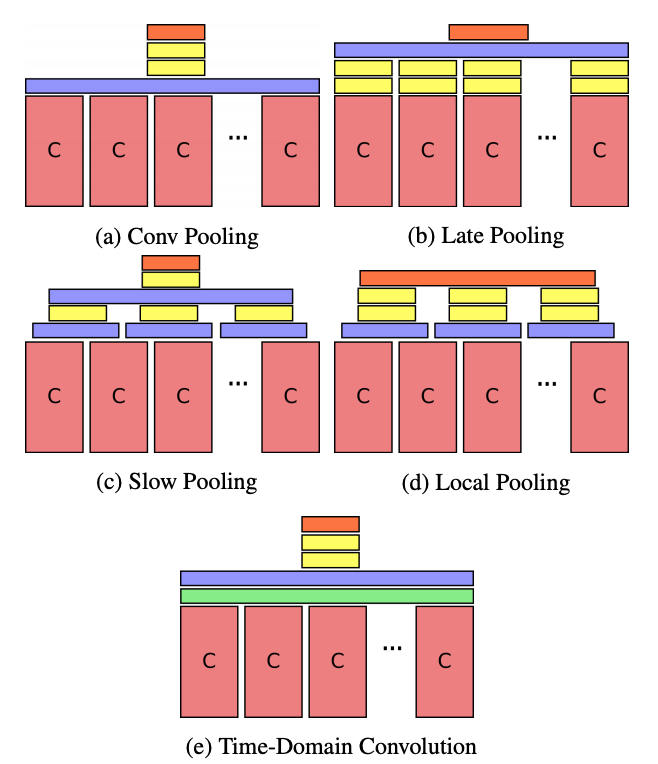
\includegraphics[width=0.7\linewidth]{fig/stacked_conv.png}
	\caption{Architecture of stacked convolution}
	\label{fig:stacked_conv}
\end{figure}

\subsection{LSTMと2DCNNの組み合わせ}
時系列解析に使われるLSTMを用いて3次元の画像を解析することができる.これはよく動画の解析で行われることがある.つまりフレームごとの画像の特徴を2次元のCNNで計算してから時系列情報をLSTMで解析することで,画像の時系列解析を行うことができる.これを3次元の医療画像でCTやMRIで適用する研究も行われている.3DCNNのデメリットであったパラメータの増大を2DCNNとLSTMの組み合わせで解決することができる.

\section{教師なし学習}
機械学習の手法には,上記で説明したように,ラベルの貼られているデータセットを用いて学習することを教師あり学習と呼び,その反対で,データセットはあっても,そのデータセットの特性を示したラベルが与えられていない場合のデータセットを用いて学習することを教師なし学習と呼ぶ.

\subsection{Autoencoder}
教師なし学習で画像の特徴を抽出する方法としてオートエンコーダがある.画像の場合におけるオートエンコーダの手法とは,ある画像から情報を圧縮する「エンコーダ」と言われる部分と,その圧縮した情報から画像を復元する「デコーダ」の二つからなる.入力とデコーダから復元された画像が同じ画像になるようにニューラルネットワークで学習させる.この学習の結果,潜在変数は似てる画像どうしで近い値になるように変化し,この分布を見れば画像の分類を教師ラベルがなくても,学習を行うことができる.

\subsection{Variational Autoencoder}
本研究では,このオートエンコーダの派生である.Variational Autoencoder(VAE)を利用した.これはオートエンコーダの「エンコーダ」と「デコーダ」は同じネットワーク構造であるが,データセットの潜在変数の分布が,正規分布になるような制約を加えて学習を行う手法である.こうすることでAutoencoderの潜在変数では分布の距離に意味ないが,VAEでは正規分布に埋め込まれるため,画像の類似度を分布が表現することができるところが特徴である.

\subsection{敵対的生成ネットワーク}
敵対的生成ネットワーク(Generative Advarsarial Network: GAN)は2014年に提案された手法である.\fig {GAN}のようにGANではGeneratorとDiscriminatorの2つのネットワークがある.Generatorは訓練データと同じような画像を生成するネットワークでDiscriminatorは,入力されたデータが訓練データから来たものかGeneratorで生成されたものかを識別するように学習する.
VAEよりもGANの方が細部まで鮮明に画像を生成することができる.しかしGANは計算時間がかかるという問題や,DiscriminatorかGeneratorのどちらかか強くなってしまうなど,学習が安定しない問題があるため,これについての多くの研究報告がされている.

\begin{figure}[H]
	\centering
	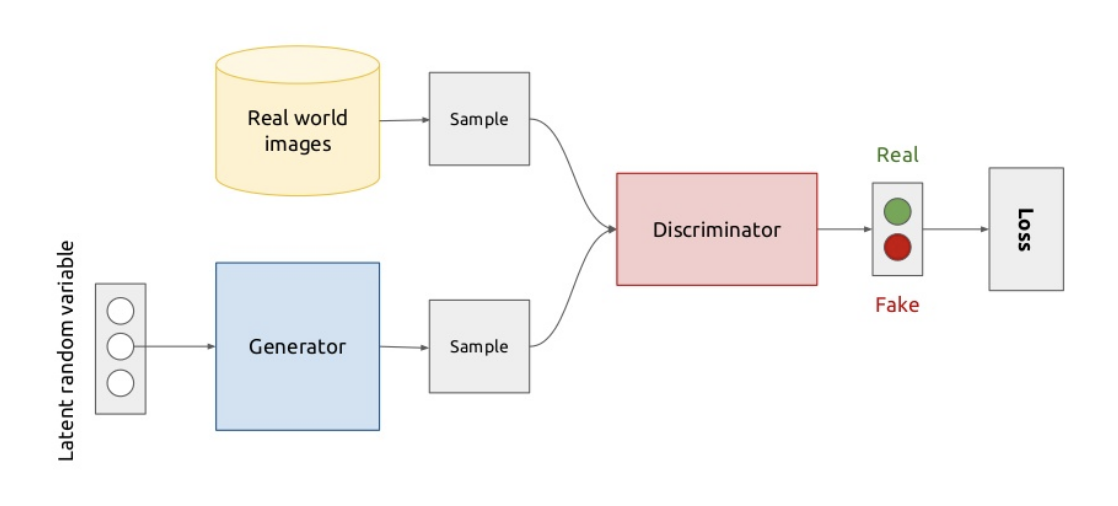
\includegraphics[width=0.7\linewidth]{fig/generative_adversarial_nets.png}
	\caption{Diagram of GAN}
	\label{fig:GAN}
\end{figure}

\section{半教師あり学習}
弱教師あり学習とも呼ばれる.これは,教師あり学習と教師なし学習を組み合わせて学習する方法である.こうすることでデータに教師ラベルをつけているものが少数であっても,データの特徴を学習しながら少量のラベルで識別境界を決めることができる.
GANやVAEの考え方を発展させてネットワークを構築することが考えられる.
 % 原理
%\chapter{自分の研究本体を述べるところ}
ここは自分のやった研究を述べる章です。実際の中身に合わせて章を複数立てにする場合もあると思います。「議論」の章を別に分ける場合は、この章では得られた結果までを記述し、その結果に対する議論は「議論」の章に回すのが良いでしょう。この章は必ずしも1つの章のみである必要はありません。研究内容に応じて、複数の章に分割することも一般的に行われます。

修士論文で大切なことは、第~\ref{chap_intro}~章や第~\ref{chap_review}~章で述べた伏線(研究の目的と動機)を回収するべく、きちんと研究内容を順序立てて書き、また自分の貢献を明確にすることです。論文全体で論理展開がきちんとしていれば良いので、必ずしも実際に行った実験などの時系列でこの章を書き進める必要はありません。また修士論文としての完成度が大切ですので、修士論文のテーマに直接関係のない自分のやったことを無理に混ぜる必要もありません。
 % 実験手法
%
\chapter{結果}\label{chap_result}
%loss,accのグラフは全て.
%前処理を行った場合は,その画像の一例も載せる
%モデルの画像(appendixの方がいいかもしれないです)
%各sectionで異なる場合は各sectionで載せましょう
%なるべくpdfで保存しましょう

\section{古典的な画像処理手法による識別精度評価}
%楕円検出の塗った画像
%円検出の画像
\begin{figure}[H]
	\centering
	\includegraphics[width=0.7\linewidth]{fig/circle_detection}
	\caption{Detection of circle.}
	\label{fig:circle_detection}
\end{figure}

\begin{figure}[H]
	\centering
	\includegraphics[width=0.7\linewidth]{fig/eclips_detection}
	\caption{Detection of ellipse}
	\label{fig:ellipse_detection}
\end{figure}

\fig{circle_detection}が円検出を利用して正常の構造を検出した結果である.緑色の円の部分が円検出された領域を示している.
真円にフィッティングしているので綺麗な円構造のみの検出となり,正常でも検出できていない部分が多くなっている.全体的に,正常領域で円検出が多く行われ,腫瘍領域では,円検出結果が少なくなる結果となったが,腫瘍部分も円検出されている部分が一部ある.

楕円検出を行った結果は\fig{ellipse_detection}で円検出よりも正常領域の検出が増えた.楕円検出がされた領域の多いところほど正常の領域で,楕円検出が少ない領域が腫瘍であるという傾向を捉えることができた.古典的な画像処理の利点は,画像検出の理由が説明できることである.このような円検出や楕円検出であれば,円形度を算出することができるので,深層学習を用いた結果よりも透明性がある.しかしながら明確な輪郭で無ければ検出できない場合が多く検出精度に限界があることから,これでは腫瘍の見落とし防止に利用することができない.そこで古典的な画像処理の性能を上回る,深層学習を利用するが必要であると分かる.

\section{教師あり学習による識別精度評価}
教師あり学習では,まず2次元画像で,元画像のまま学習した場合と,擬似HE変換した画像を学習する場合,さらに事前学習を行った場合で比較を行った.
\begin{figure}
	\centering
	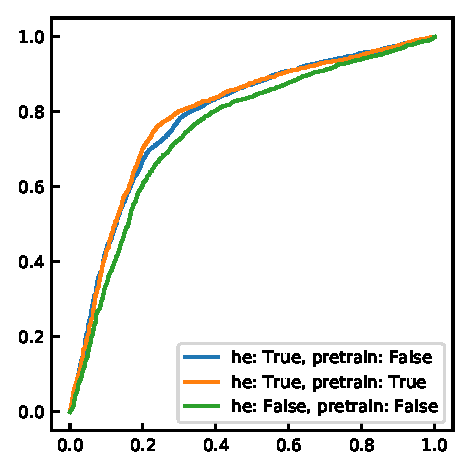
\includegraphics[width=0.6\linewidth]{fig/chapter4/2dcnn_preprocessing}
	\caption{2DCNN with different preprocessing}
	\label{fig:2dcnnpreprocessing}
\end{figure}

\begin{figure}
	\centering
	\begin{minipage}[b]{0.45\columnwidth}
	\centering
	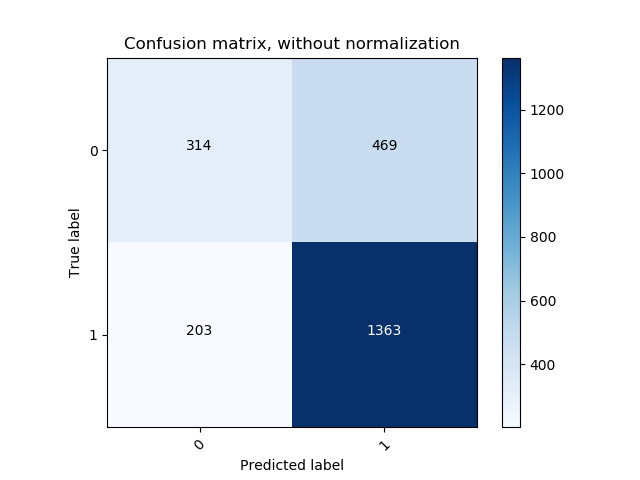
\includegraphics[clip, width=\linewidth]{fig/chapter4/count_pretrain_False_he_False}
	\subcaption{pretrain: Flase, he transform: False}
	\label{fig:count_no_preprocess}
    \end{minipage}
	\begin{minipage}[b]{0.45\columnwidth}
		\centering
		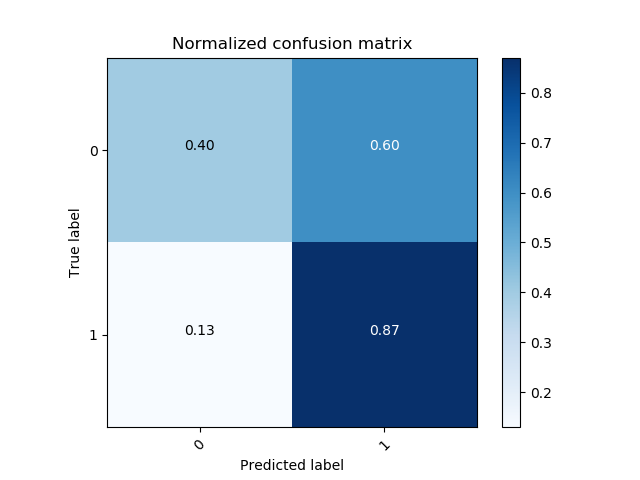
\includegraphics[clip, width=\linewidth]{fig/chapter4/pretrain_False_he_False}
		\subcaption{pretrain: Flase, he transform: False}
		\label{fig: no_preprocess}
	\end{minipage}
	\begin{minipage}[b]{0.45\columnwidth}
	\centering
	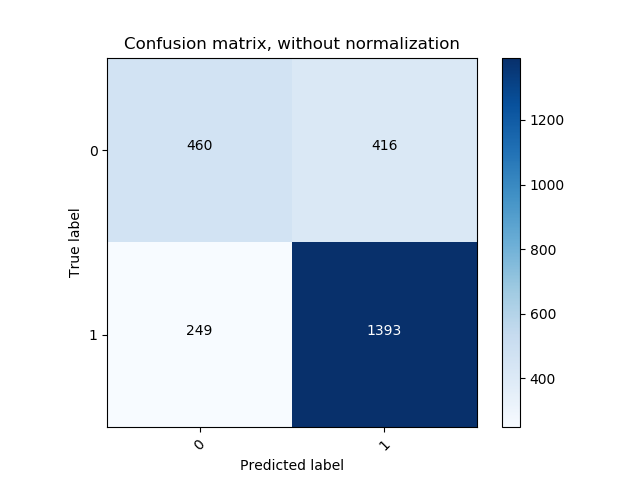
\includegraphics[clip, width=\linewidth]{fig/chapter4/count_pretrain_False_he_True}
	\subcaption{pretrain: Flase, he transform: True}
	\label{fig: count_he_preprocess}
    \end{minipage}
	\begin{minipage}[b]{0.45\columnwidth}
		\centering
		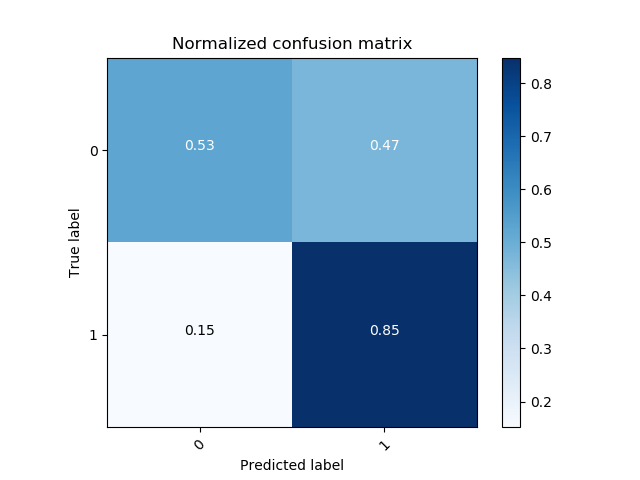
\includegraphics[clip, width=\linewidth]{fig/chapter4/pretrain_False_he_True}
		\subcaption{pretrain: Flase, he transform: True}
		\label{fig: he_preprocess}
	\end{minipage}
	\begin{minipage}[b]{0.45\columnwidth}
	\centering
	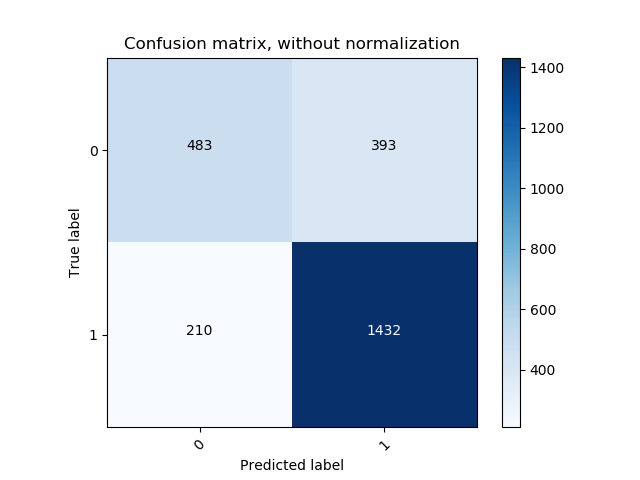
\includegraphics[clip, width=\linewidth]{fig/chapter4/count_pretrain_True_he_True}
	\subcaption{pretrain: True, he transform: True}
	\label{fig: count_pretrain_preprocess}
    \end{minipage}
	\begin{minipage}[b]{0.45\columnwidth}
		\centering
		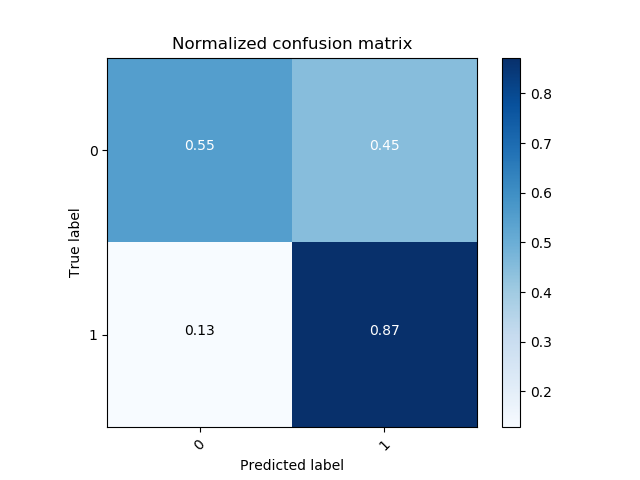
\includegraphics[clip, width=\linewidth]{fig/chapter4/pretrain_True_he_True}
		\subcaption{pretrain: True, he transform: True}
		\label{fig: pretrain_preprocess}
	\end{minipage}

	
	\caption{Confusion Matrix for 2DCNN with different preprocessing}
	\label{fig:2d_preprocess_matrix}
	
\end{figure}

前処理を何も行わない場合が\fig{2dcnnpreprocessing}の緑のプロットでありROCの評価指数である.AUCはhogeで一番認識精度が低かった.また\fig{no_preprocess}のように腫瘍は87\%の精度で検出できているが,正常は40\%の精度でしか検出できていなかった.

ここで腫瘍の見落としとなる偽陰性の割合が13\%と低く,偽陽性が高くなっていることが分かる.このようになった理由は,深層学習の学習方法に理由がある.今回学習に用いたデータで正常は,783枚であるのに対して,腫瘍の学習データの枚数は1566枚である.正常の画像よりも腫瘍の画像を2倍多く学習に利用することで,腫瘍の検出がより重要視されるモデルになったのである.これは,病変の見落としリスクを防止するためには,非常に良い結果となった.

腫瘍の見落とし率が低いことは良いが,正常を腫瘍と判断する割合が高すぎるのでこれを正しく正常画像を正常と判断できるようにしなくてはならない.

ここで前処理として擬似HE変換を行って学習した結果(\fig{he_preprocess})と,擬似HE変換した後に,事前学習も行った時の学習結果(\fig{pretrain_preprocess})から,前処理をすることで腫瘍の見落としリスクを低くしたまま,正常画像を正しく認識することができるようになった.

\subsection*{モデルの比較}
InceptionV3とXception, InceptionResnetV2を比較して,どのネットワークが認識精度が高いのかを実験した.

\subsection{3次元画像解析}
3DCNNは,学習する際の訓練パラメータが多すぎて,学習が収束しない点や,メモリが大きくてGPUに乗らないという問題があり,時系列解析で行われているLSTMやGRUまた,BidirectionalなGRUをモデルの比較として利用した.

\begin{figure}
	\centering
	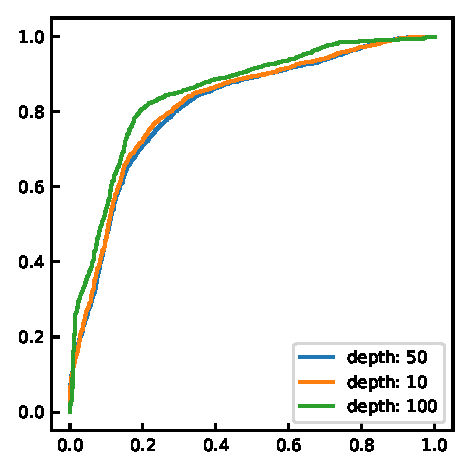
\includegraphics[width=0.7\linewidth]{fig/chapter4/3d/roc/depth_all.pdf}
	\caption{depth}
	\label{fig:depthall}
\end{figure}

\begin{figure}[H]
	\centering
	
	\begin{minipage}[b]{0.45\columnwidth}
		\centering
		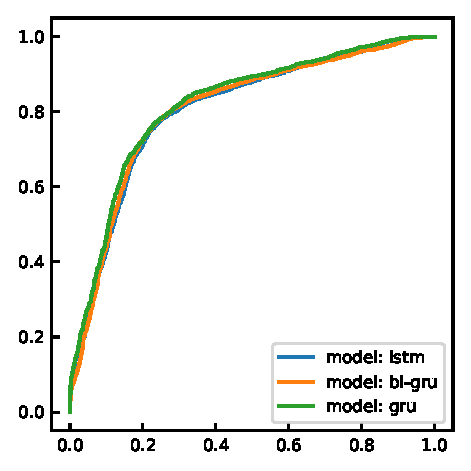
\includegraphics[clip, width=\linewidth]{fig/chapter4/3d/roc/depth_10.pdf}
		\subcaption{depth: 10}
		\label{fig:}
	\end{minipage}
	\begin{minipage}[b]{0.45\columnwidth}
		\centering
		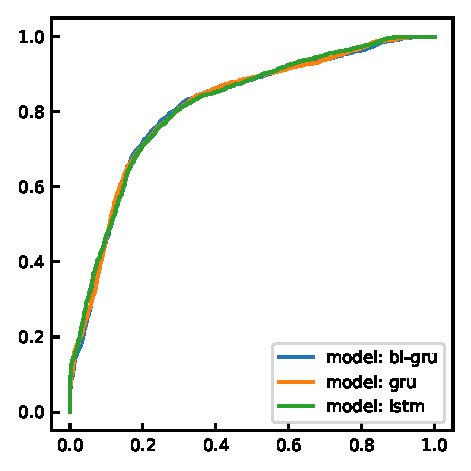
\includegraphics[clip, width=\linewidth]{fig/chapter4/3d/roc/depth_50.pdf}
		\subcaption{depth: 50}
		\label{fig:}
	\end{minipage}
	\begin{minipage}[b]{0.45\columnwidth}
		\centering
		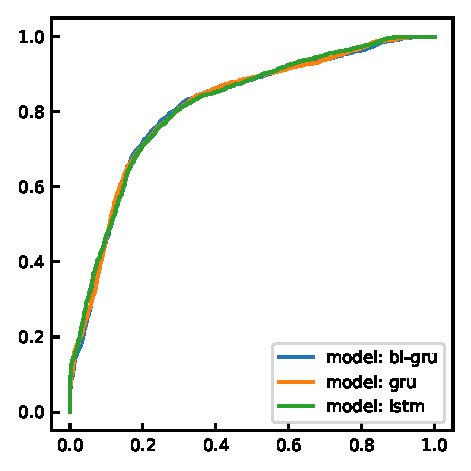
\includegraphics[clip, width=\linewidth]{fig/chapter4/3d/roc/depth_100.pdf}
		\subcaption{depth: 100}
		\label{fig:}
	\end{minipage}
	
	\caption{ROC curve with different depth}
	\label{fig:2dcnn+LSTM_roc}
	
\end{figure}

\section{教師なし学習による識別精度評価}
\subsection{Auto Encoder}
\begin{figure}
	\centering
	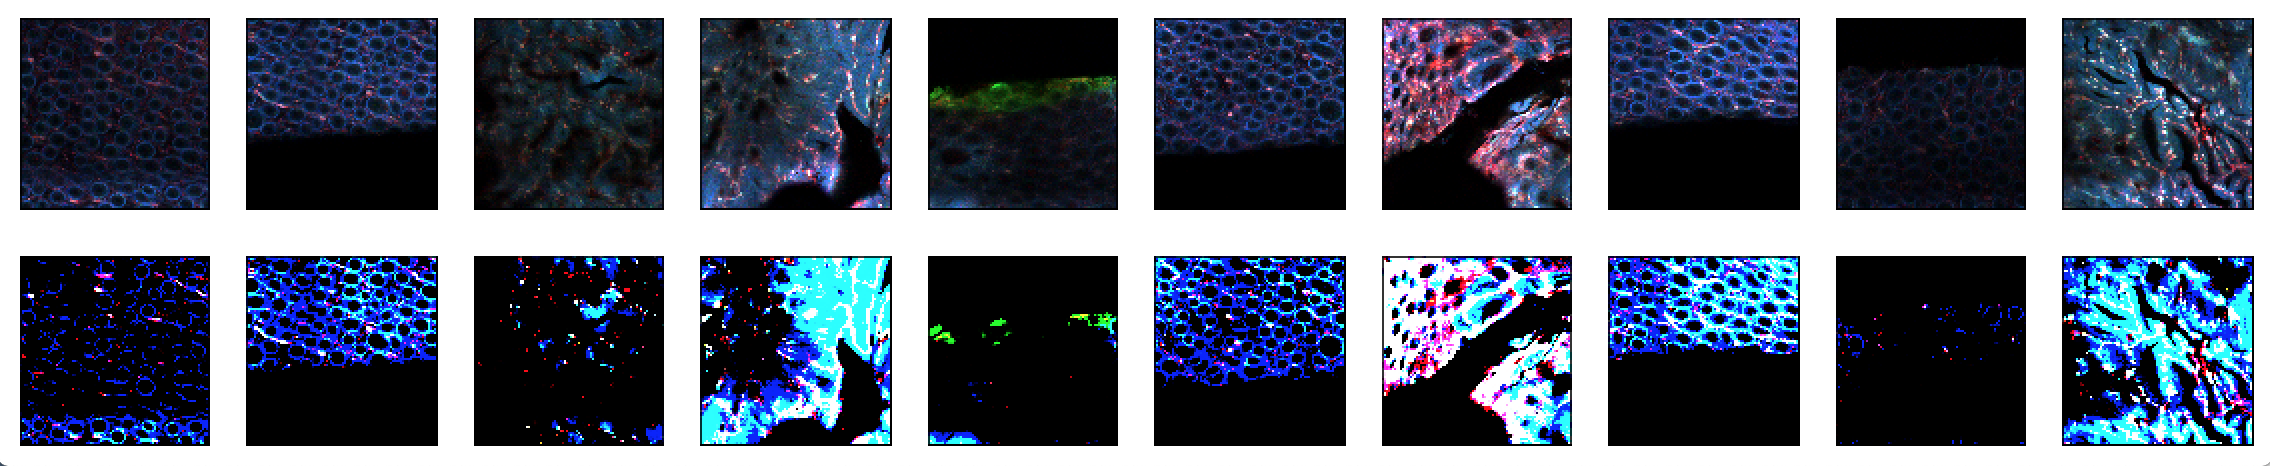
\includegraphics[width=0.9\linewidth]{fig/chapter4/unet_ae}
	\caption{Auto Encoder}
	\label{fig:unetae}
\end{figure}

\subsection{GAN}

\begin{figure}[H]
	\centering
	
	\begin{minipage}{0.24\columnwidth}
		\centering
		
\includegraphics[clip, width=\linewidth]{fig/generative_adversarial_nets/0000_0000}
		\subcaption{epochs = 0}
		\label{fig:}
	\end{minipage}
	\begin{minipage}{0.24\columnwidth}
		\centering
		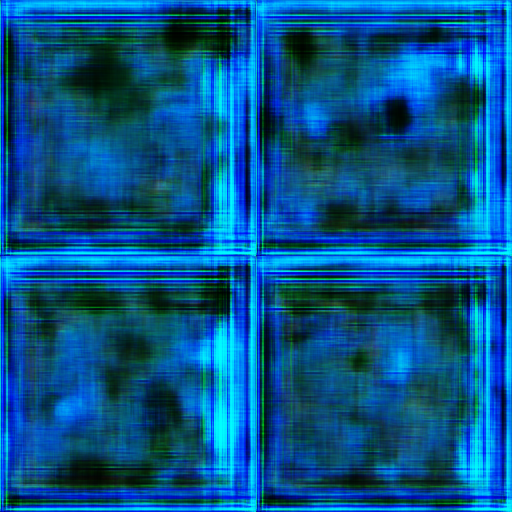
\includegraphics[clip, width=\linewidth]{fig/generative_adversarial_nets/0079_0000}
		\subcaption{epochs = 79}
		\label{fig:}
	\end{minipage}
	\begin{minipage}{0.24\columnwidth}
		\centering
		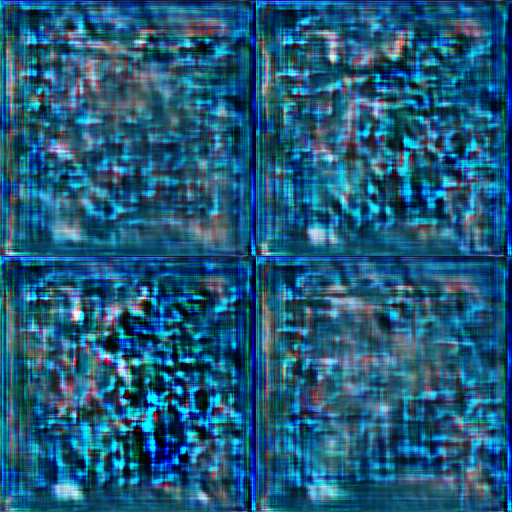
\includegraphics[clip, width=\linewidth]{fig/generative_adversarial_nets/0641_0000}
		\subcaption{epochs = 641}
		\label{fig:}
	\end{minipage}
	\begin{minipage}{0.24\columnwidth}
		\centering
		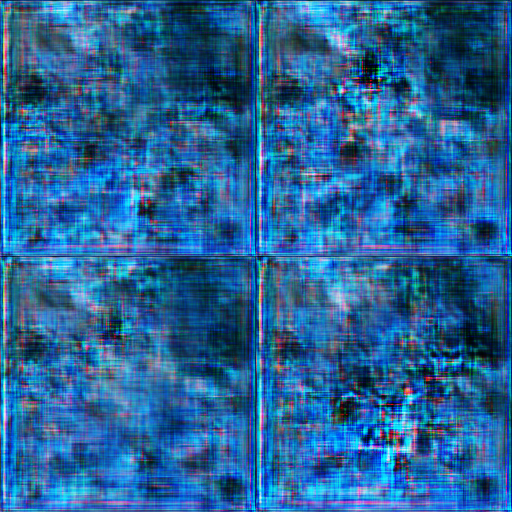
\includegraphics[clip, width=\linewidth]{fig/generative_adversarial_nets/0969_0000}
		\subcaption{epochs = 969}
		\label{fig:}
	\end{minipage}
	\begin{minipage}{0.24\columnwidth}
		\centering
		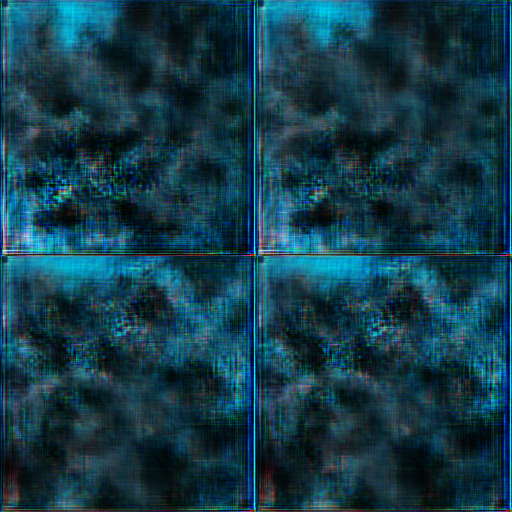
\includegraphics[clip, width=\linewidth]{fig/generative_adversarial_nets/1213_0000}
		\subcaption{epochs = 1213}
		\label{fig:}
	\end{minipage}
	\begin{minipage}{0.24\columnwidth}
		\centering
		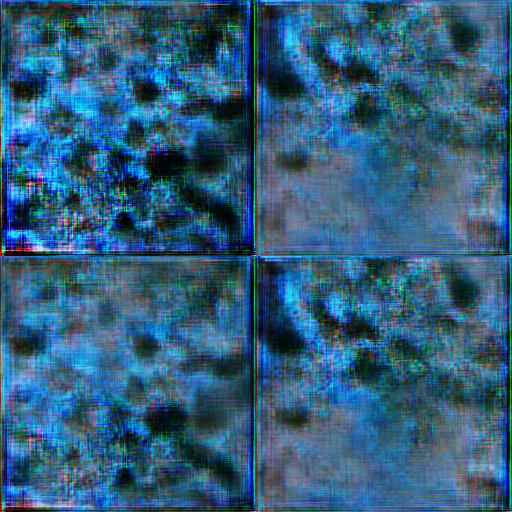
\includegraphics[clip, width=\linewidth]{fig/generative_adversarial_nets/1619_0000}
		\subcaption{epochs = 1619}
		\label{fig:}
	\end{minipage}
	\begin{minipage}{0.24\columnwidth}
		\centering
		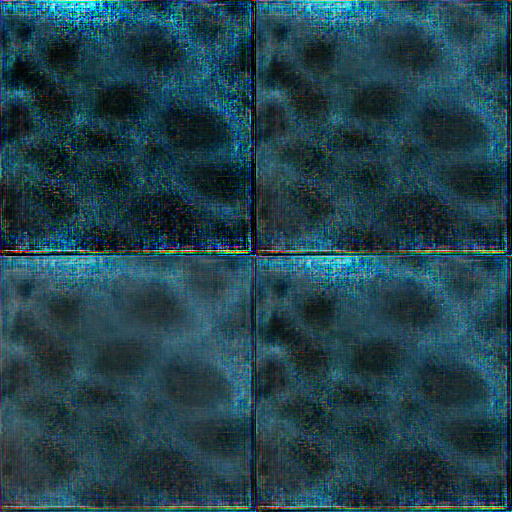
\includegraphics[clip, width=\linewidth]{fig/generative_adversarial_nets/2004_0000}
		\subcaption{epochs = 2004}
		\label{fig:}
	\end{minipage}
	\begin{minipage}{0.24\columnwidth}
		\centering
		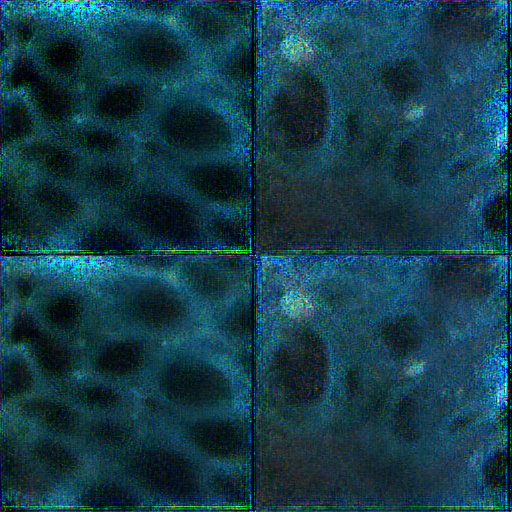
\includegraphics[clip, width=\linewidth]{fig/generative_adversarial_nets/3208_0000}
		\subcaption{epochs = 3208}
		\label{fig:}
	\end{minipage}
	
	\caption{Transition generated images by GAN}
	\label{fig:GANimage}
	
\end{figure}

\subsection{VAE}
擬似HE染色した画像と元のカラー画像のそれぞれに対してVAEを行い,潜在変数を2次元空間にプロットした結果を\fig {VAEplot}に示す.
\begin{figure}[H]
	\centering
	
	\begin{minipage}[b]{0.45\columnwidth}
		\centering
		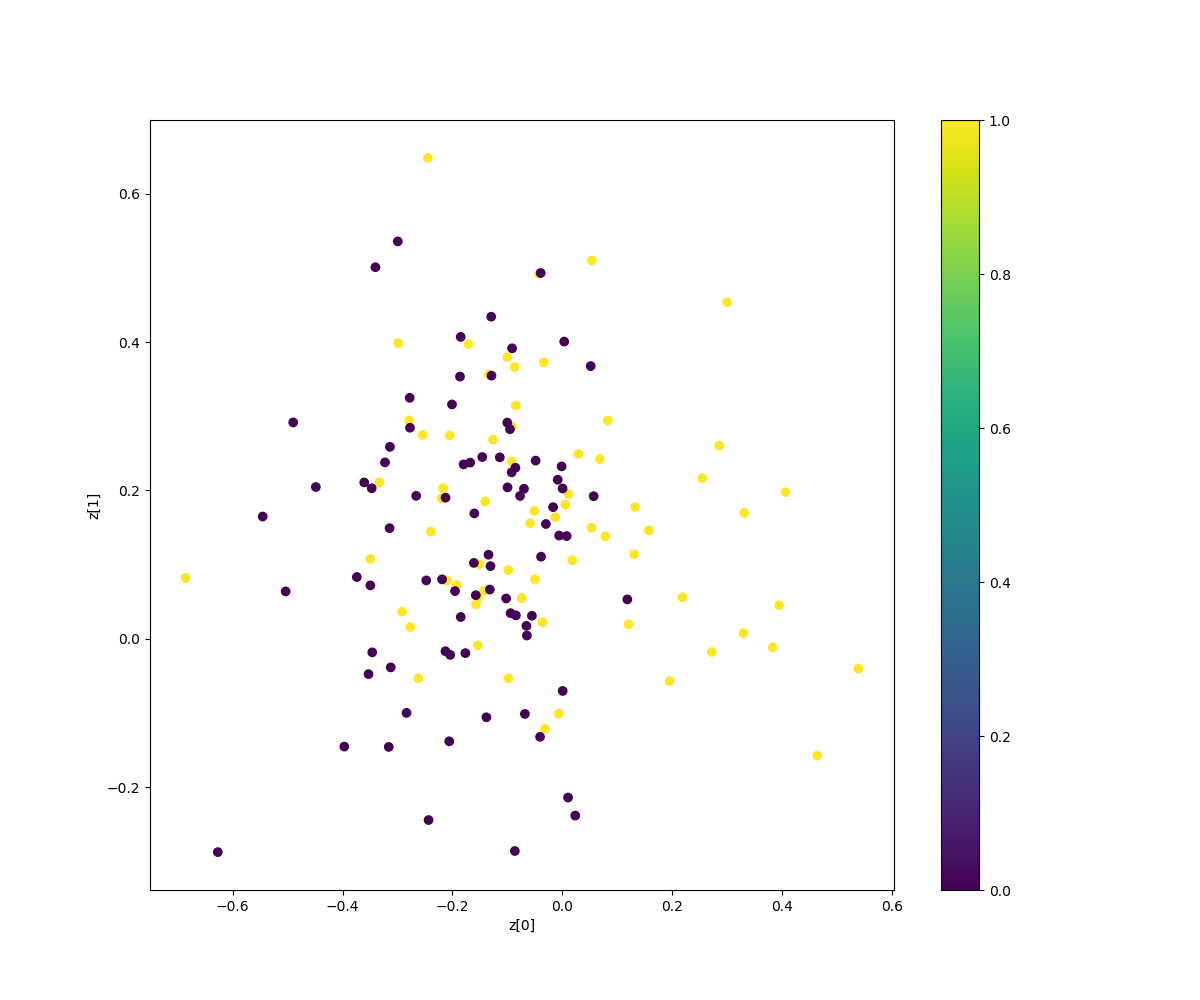
\includegraphics[clip, width=\linewidth]{fig/variational_auto_encoder/vae_colon_epoch_100_c13_he}
		\subcaption{HE like color at sample A}
		\label{fig:}
	\end{minipage}
	\begin{minipage}[b]{0.45\columnwidth}
		\centering
		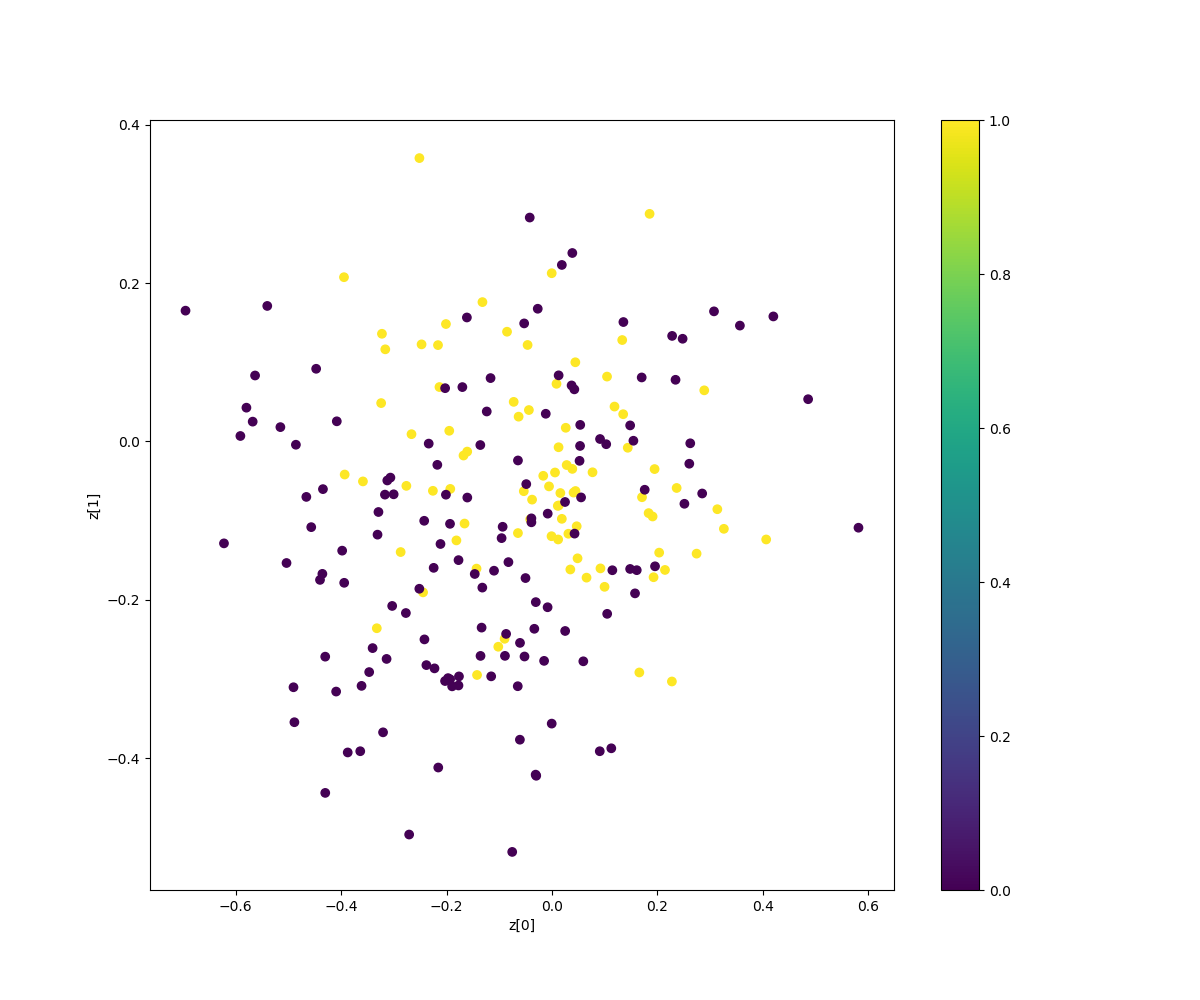
\includegraphics[clip, width=\linewidth]{fig/variational_auto_encoder/vae_colon_epoch_299_c13_rgb}
		\subcaption{original color at sample A}
		\label{fig:}
	\end{minipage}
	\begin{minipage}[b]{0.45\columnwidth}
		\centering
		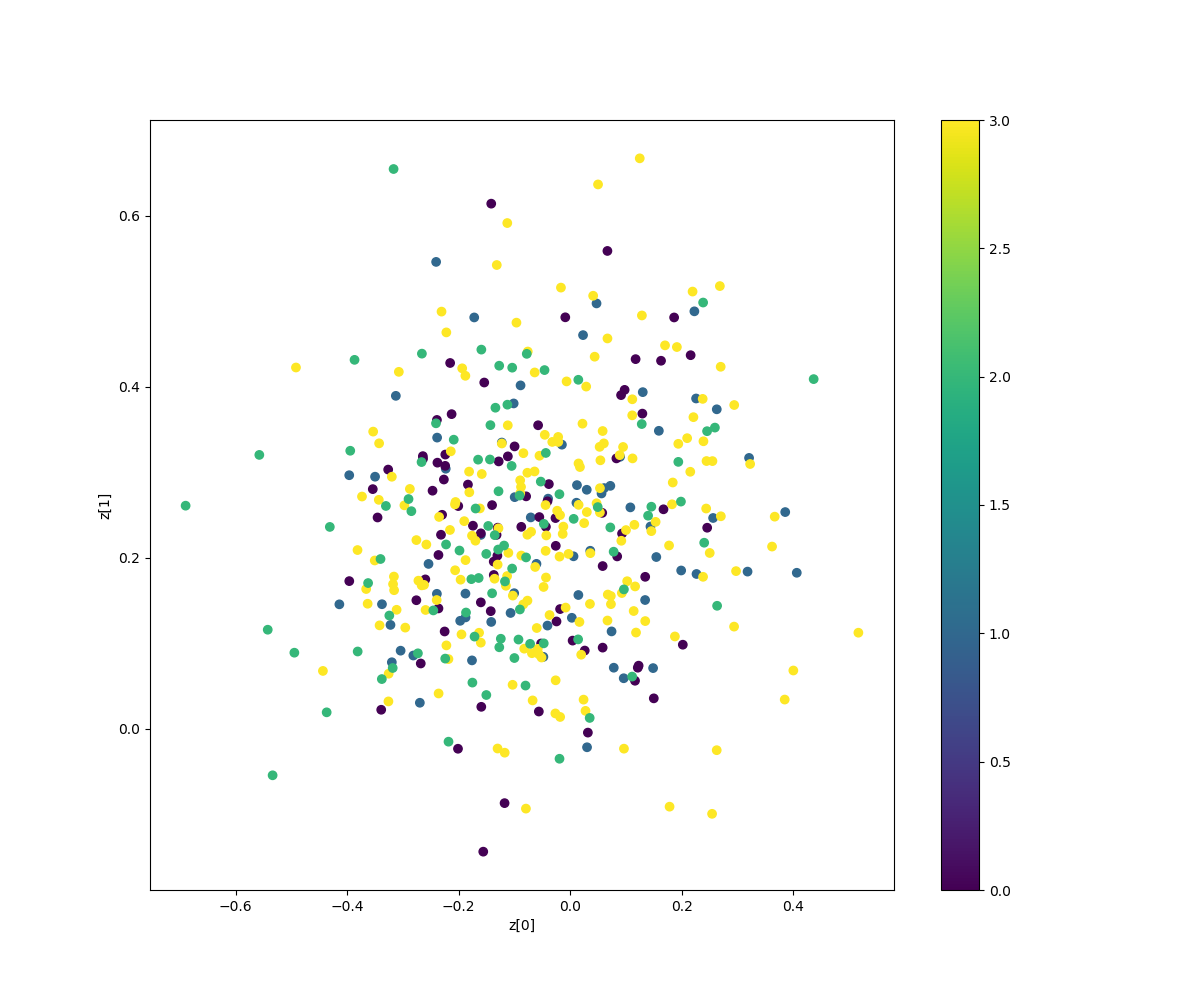
\includegraphics[clip, width=\linewidth]{fig/variational_auto_encoder/vae_colon_epoch_100_he_mix}
		\subcaption{HE like color at sample A and B}
		\label{fig:}
	\end{minipage}
	\begin{minipage}[b]{0.45\columnwidth}
		\centering
		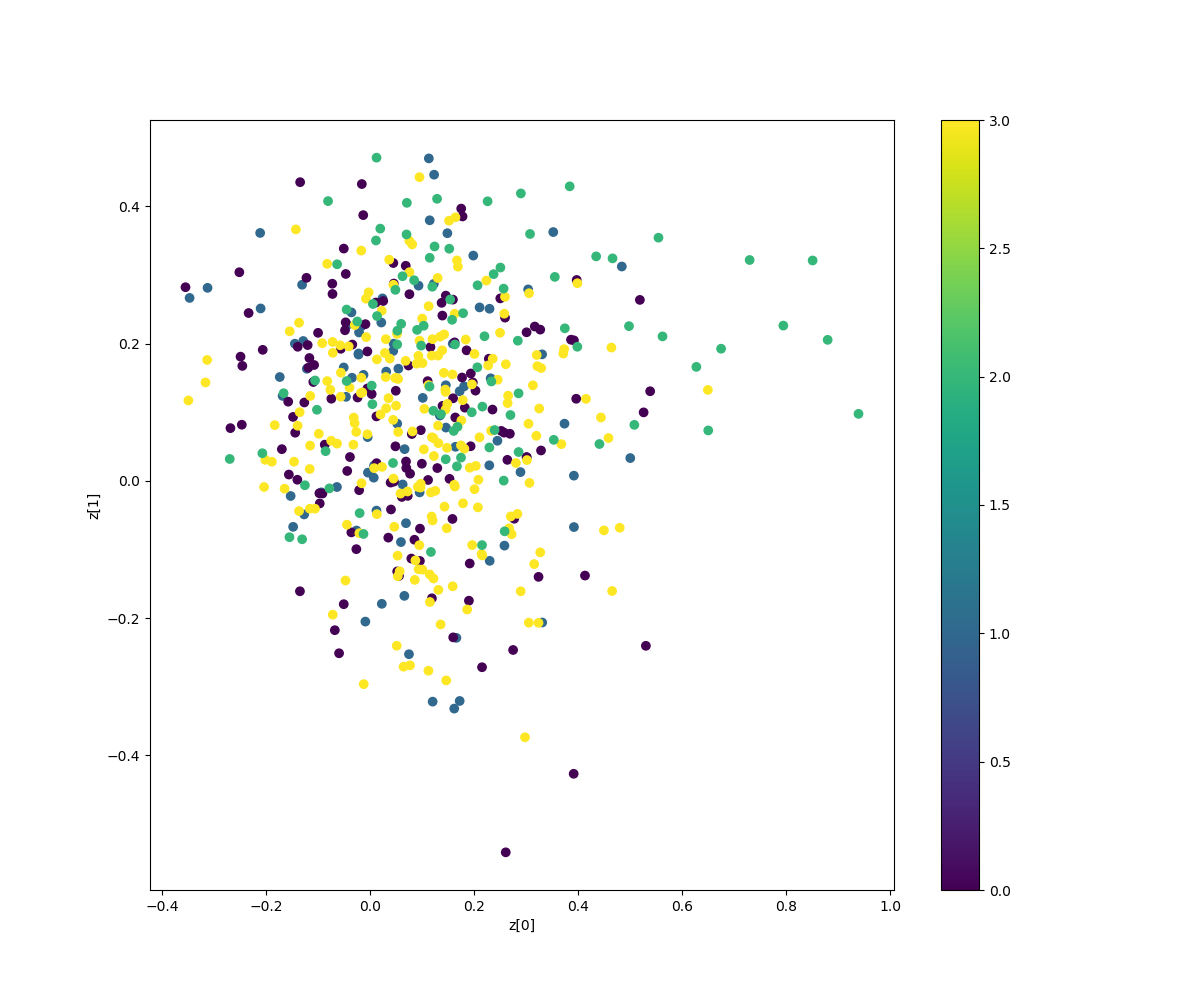
\includegraphics[clip, width=\linewidth]{fig/variational_auto_encoder/vae_colon_epoch_100_rgb_mix}
		\subcaption{original color at sample A and B}
		\label{fig:}
	\end{minipage}
	
	\caption{Latent space of 2D. Color ratio 1 is cancer, 0 is normal.}
	\label{fig:VAEplot}
	
\end{figure}

部分的には,正常と腫瘍で分布が異なるようになったが,明確な境界線を引くことが難しい.したがって,教師あり学習で境界を明確にし,教師なし学習でデータの構造を抽出することができれば,もっとも精度の高い認識モデルが作れる.

\section{半教師あり学習による識別精度評価}
\begin{figure}
	\centering
	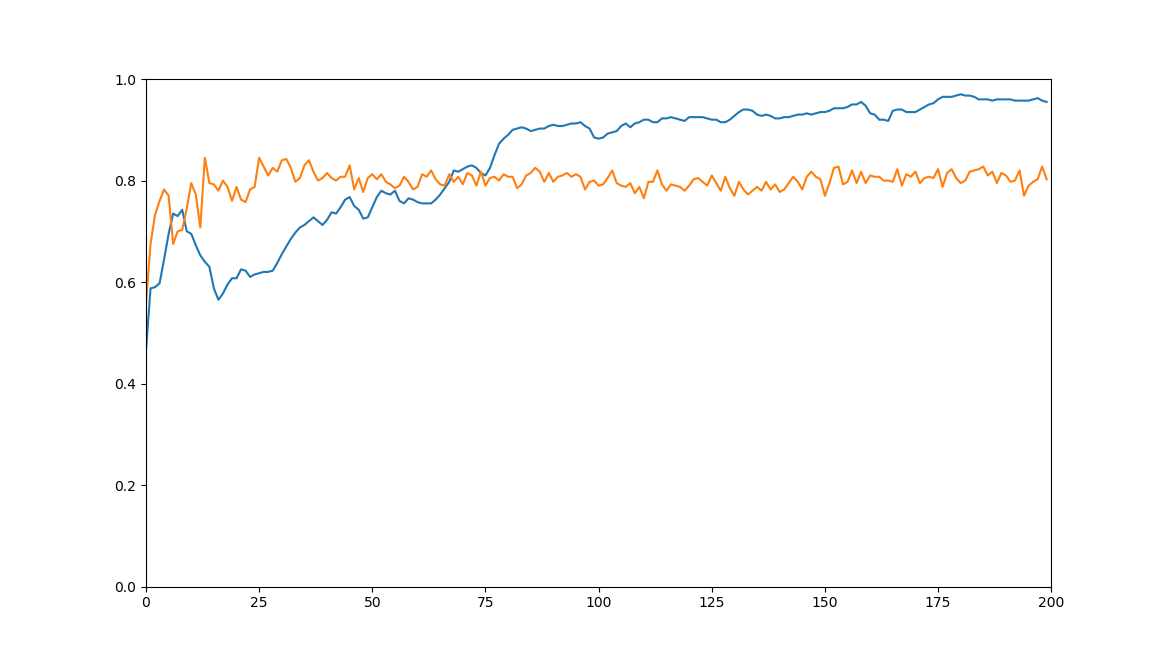
\includegraphics[width=0.7\linewidth]{fig/chapter4/accuracy_summary}
	\caption{VAE Accuracy}
	\label{fig:accuracysummary}
\end{figure}



\section{学習結果の可視化}
深層学習を用いて,腫瘍らしい領域を認識するアルゴリズムを,病理医が見るために画像上に腫瘍の部分が見て分かるように可視化を行った.

スライドウィンドウで

Grad-CAMを利用することでより詳細に深層学習の判断が可視化されるようになった.
\begin{figure}
	\centering
	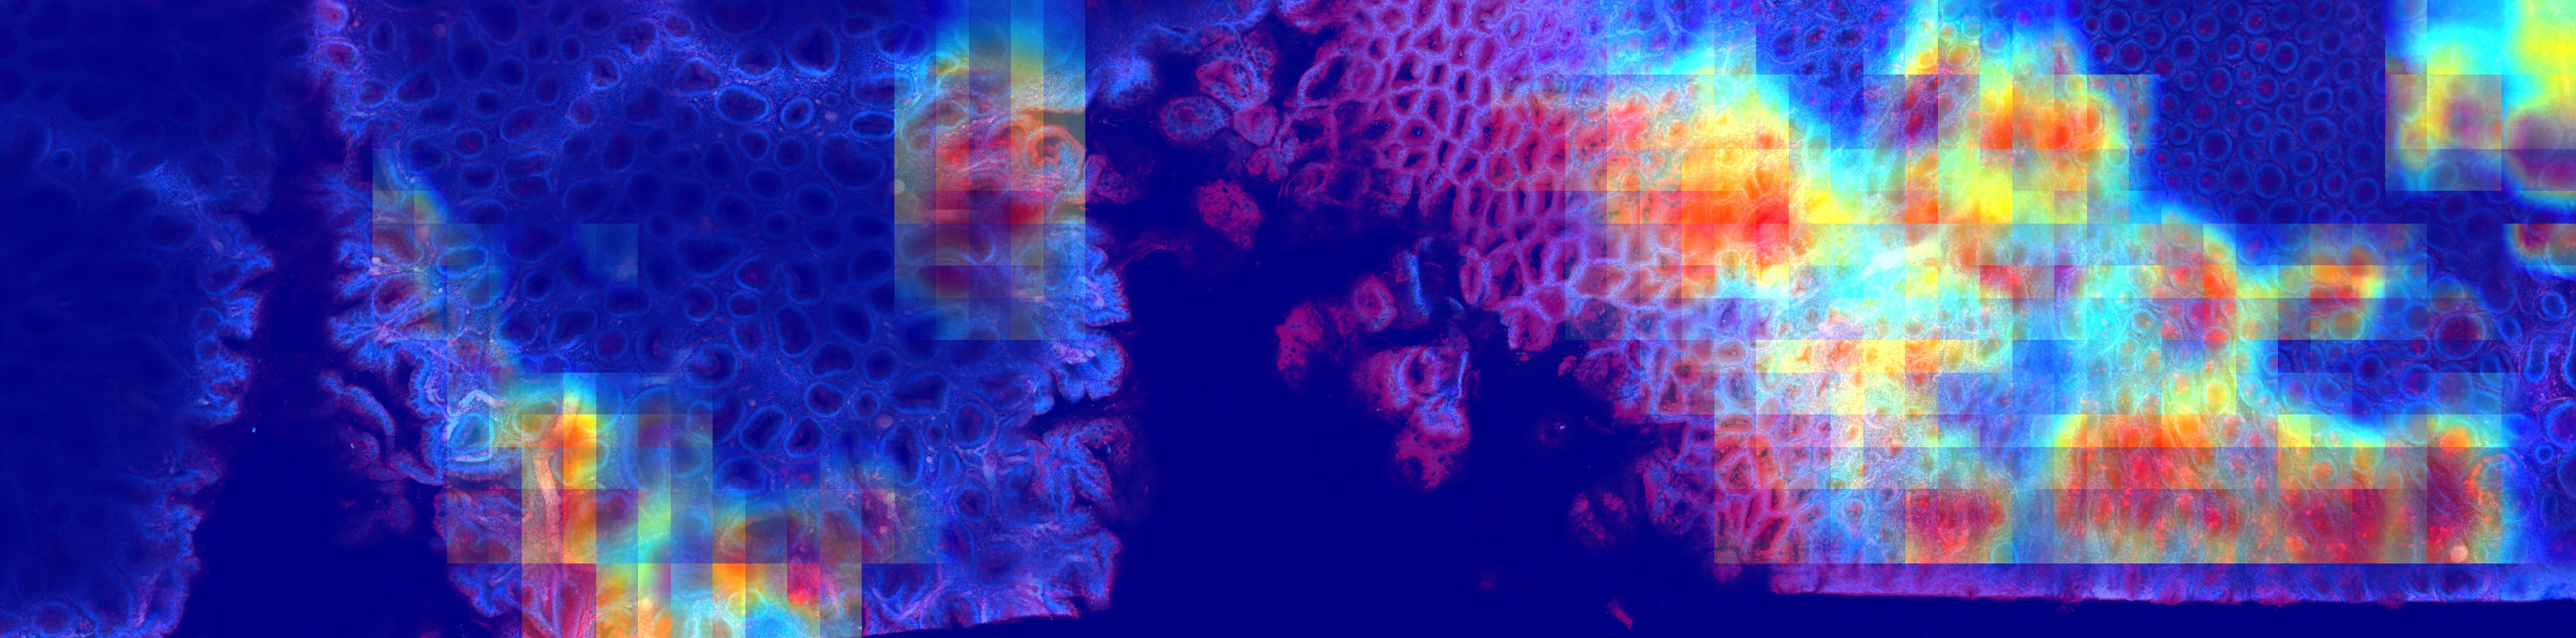
\includegraphics[width=0.7\linewidth]{fig/chapter4/large-grad-cam-step100-rm-black}
	\caption{Visualization with Grad-CAM}
	\label{fig:large-grad-cam-step100-rm-black}
\end{figure}
 % 結果と考察
%\chapter{結論}
まとめと今後の展望
 % まとめ
%\chapter*{付録} % 章番号を出さない
\addcontentsline{toc}{chapter}{付録} % 目次に載せる

「付録」(appendix)は、論文の本文に載せるには情報として邪魔もしくは必須ではないものの、読者にとって有益となるような情報を載せます。付録を必要としない論文ももちろん存在しますので、そこは著者の判断です。

例えば、たくさんの観測データを様々なモデルでフィットした場合、フィット結果の絵がたくさん出てくるはずです。そのような図は本文中に大量に出されても大切な情報を見失ってしまいますので、大部分は付録に載せることが推奨されます。他には、何かしらの長い式変形や証明を載せる必要がある場合、付録に移動する場合があります。

% 付録は chapter の 1 つとして作りますが、章番号は表示しません。
% また付録の 1 つずつはアルファベットで番号付けをするのが一般的です。
\setcounter{section}{0} % section の番号をゼロにリセットする
\renewcommand{\thesection}{\Alph{section}} % 数字ではなくアルファベットで数える
\setcounter{equation}{0} % 式番号を A.1 のようにする
\renewcommand{\theequation}{\Alph{section}.\arabic{equation}}
\setcounter{figure}{0} % 図番号
\renewcommand{\thefigure}{\Alph{section}.\arabic{figure}}
\setcounter{table}{0} % 表番号
\renewcommand{\thetable}{\Alph{section}.\arabic{table}}

\section{すごい長い証明}
式~(\ref{eq})のように、式番号がアルファベットとアラビア数字の組み合わせになるように、\LaTeX{}ソース中で設定してありますので、中身を眺めてみてください。

\begin{equation}
  \label{eq}
  1 + 1 = 2
\end{equation}


\section{すごいたくさんのフィットの図}
 % 付録
\chapter*{謝辞}%
\addcontentsline{toc}{chapter}{謝辞}%

小野寺宏 特任教授\\
指導教員として2年間ご指導いただきました.充実した研究環境を与えていただき,また幅広い先生のご紹介をしてくださり研究の異分野連携の重要性を知ることができました.毎週研究の進捗の報告でご指導いたたき,研究に行き詰まってもアイディアをたくさんいただき,研究を進めることができました.研究だけでなく今後の進路についてや医療業界の知識などを普段から教えていただき人生の選択肢を広げることができました.大変ありがとうございました.

染谷隆夫 教授\\
研究の進捗の発表の場を定期的に設けていただき,研究で困っていた部分や疑問に思うところについて染谷研究室の学生を含め,ディスカッションをすることができ,研究を前に進めることができました.大変ありがとうございました.

横田和之 講師\\
実験TAでは,電子回路の深い知識と考察や,実験の注意点を丁寧に教えていただきました.また機械学習についてのディスカッションをして理解を深めるきっかけとなりました.大変ありがとうございました.

小野敏嗣 助教\\
内視鏡生検の検体をいただき,検体の特徴だけでなく,内視鏡生検の知識や経験を教えていただき解析方法の検討に役立てることができました.また実際の内視鏡生検に立ち会わせていただき,現場の様子を見ることで,どのように研究成果を利用していくかを構想することができました.大変ありがとうございました.

長沼和則 特任研究員\\
本研究の標本処理システムの構築についてアドバイスをいただき,研究を進めることができました.大変ありがとうございました.

添田建太郎 特任研究員\\
本研究の生検検体の染色と透明化を自動処理するためのマイクロチップ作成において,とても細かい造形にこだわって作ってくださりました.大変ありがとうございました.

原田達也 教授\\
画像処理の知識をご教授いただき,医療画像の解析データについて,人が見やすい画像にすることは機械学習にとっても判断しやすくなるという助言をいただき,その後の研究に役立てることができました.大変ありがとうございました.

牛久祥孝 講師\\
本研究の画像取得方法が従来のHE染色方法とは異なるため,解析に困っていたころ,色空間を変換して擬似的なHE染色の画像に変換したことが,病理医にとって見やすいとの助言をいただき,これで機械学習でも処理することが重要であると分かりました.大変ありがとうございました.

武田伊織 特任研究員\\
3Dプリンターの使い方を丁寧に教えていただいたり,日々の研究で困っている時にアイディアをいただきました.また研究以外でも昼食に出かけて大学生活の悩みをスッキリさせることができました.発表資料の作成については,学会発表や研究発表の際に,たくさんご指導していただきました.大変ありがとうございました.

樽茶好彦 様\\
修士1年の際に,研究室の先輩として研究の相談だけでなく,修士過程の過ごし方や研究の進め方,就職についてご指導いただきました.大変ありがとうございました.

山田敦史 君\\
研究や大学生活において辛い時期でも相談に乗ってくれ,研究へのモチベーションを維持することができました.また研究テーマでお互いに機械学習を利用していたため,遅い時間まで研究のディスカッションに付き合ってくれました.大変ありがとうございました.

水谷浩哉 様\\
消化器内科の基本的な知識を教えていただきました.検体の説明を丁寧にしてくださり,本研究の解析データを正しく理解することができました.大変ありがとうございました.

福田圭佑 様\\
機械学習のプログラミングを丁寧に教えていただきました.また困った時には,アイディアからコードのレビューまで相談に乗ってくださり,研究を進めることができました.大変ありがとうございました.

鷹野玲美 学術支援専門職員\\
研究で必要な解析や画像取得などで,作業のお願いをしてから実行までがとても早く大変助かりました.また日々の研究生活で気遣ってくださり,精神的にも支えてくださりました.大変ありがとうございました.

田中麻美 技術員\\
研究の相談に乗ってくださり,普段からの雑談で研究をする元気を与えてくれました.大変ありがとうございました.

藤平まなみ 技術員\\
擬似HEの画像変換など,研究の処理で必要になった作業などをお願いしてお手伝いいただきました.大変ありがとうございました.
\\
\\
両親や友人には,健康に気を使ってくれたり様々な面で支えていただきました.ありがとうございました.
 % 謝辞

\renewcommand{\bibname}{引用文献}
\bibliographystyle{elsart-num}
\bibliography{thesis}
\label{page:bib}

\end{document}
